% Plantilla realizada por Alberto Brunete (UPM).

%Parametros de tipo libro
\documentclass[10pt,a4paper]{book}

%Idioma español y acentos
\usepackage[spanish, es-tabla]{babel}
%\usepackage[latin1]{inputenc}
\usepackage[utf8]{inputenc}

%algunos sÌmbolos matemáticos y paquetes para usar subimágenes
\usepackage{amsmath}
\usepackage{amsfonts}
\usepackage{amssymb}
\usepackage{graphicx}
\usepackage[export]{adjustbox}
%\usepackage{subfigure}
\usepackage{subcaption}
\usepackage{listings}
\usepackage{appendix}
\usepackage{float}
\usepackage{array}
%Márgenes
\usepackage[left=3cm,top=3cm,right=3cm,bottom=3cm]{geometry}

%
\usepackage{multicol}
\usepackage{multirow}

%para generar índice con hipervínculos
\usepackage{hyperref}

%parametros del documento (sus propiedades)
\hypersetup{
    pdftitle={José Luis Grande Morón - TFG - 2019},
    pdfsubject={TFG - 2019},
    pdfauthor={José Luis Grande Morón},
    pdfkeywords={XBee} {Domótica} {brazo robótico},
    colorlinks,
    citecolor=black,
    filecolor=black,
    linkcolor=black,
    urlcolor=black,
}
 
%Código
\usepackage{listings}
%Rename Listlings
\renewcommand{\lstlistingname}{Código}% Listing -> Algorithm
\renewcommand{\lstlistlistingname}{Lista de \lstlistingname s}
\renewcommand{\labelitemii}{$-$}
% List of Listings -> Lista de Código

%Debug
%\DeclareUnicodeCharacter{0301}{*************************************}

%empieza el documento
\begin{document}  

%elementos antes del trabajo en sÌ se meten dentro de frontmatter
\frontmatter

%cada incluye referencia a un archivo de tipo .tex
\begin{titlepage}
\begin{center}

%forma de introducir imágenes. el \\[0.5 cm] de final de línea introduce un salto de ese tamaño.
%width=1\textwidth indica el tamaño de la imágen (valores entre 0-1). 
 
\includegraphics[width=1\textwidth]{figuras/cabecera.png}  \\[0.5 cm]

\LARGE UNIVERSIDAD POLITÉCNICA DE MADRID \\ [1 cm]

\LARGE ESCUELA TÉCNICA SUPERIOR DE INGENIERÍA Y DISEÑO INDUSTRIAL \\ [1 cm]

\LARGE Grado en Ingeniería Electrónica y Automática Industrial\\ [1 cm]

\LARGE \textbf{TRABAJO FIN DE GRADO}\\[1 cm]

\Huge \textsc{Título del trabajo}\\[1 cm]

\LARGE Autor \\[2 cm]

%flushleft alinea a la izquierda el texto

\begin{multicols}{2} 
\begin{flushleft} \Large
\emph{Cotutor (si lo hay):} nombre y apellidos \\
\emph{Departamento:} departamento
\end{flushleft}

\begin{flushleft} \Large
\emph{Tutor:} nombre y apellidos\\
\emph{Departamento:} departamento
\end{flushleft}

\end{multicols} 

%rellena de blanco el resto de la página para escribir abajo del todo
\vfill

% Bottom of the page
{\large Ciudad, Mes, Año}

%SE ponen al final firmas.tex
%\end{center}
%\end{titlepage}


\cleardoublepage 

%\begin{center}
% Está puesto en portada.tex
\thispagestyle{empty}
%forma de introducir imágenes. el \\[0.5 cm] de final de línea introduce un salto de ese tamaño.
%width=1\textwidth indica el tamaño de la imágen (valores entre 0-1). 

\includegraphics[width=1\textwidth]{figuras/cabecera.png}  \\[0.5 cm]

\LARGE UNIVERSIDAD POLITÉCNICA DE MADRID \\ [1 cm]

\LARGE ESCUELA TÉCNICA SUPERIOR DE INGENIERÍA Y DISEÑO INDUSTRIAL \\ [1 cm]

\LARGE Grado en Ingeniería Electrónica y Automática Industrial\\ [1 cm]

\LARGE \textbf{TRABAJO FIN DE GRADO}\\[1 cm]

\Huge \textsc{Conexion de RoboHealthArm a una red domotica empleando radiofrecuencia}\\[2 cm]

\Large Firma Autor \\[3 cm]

%flushleft alinea a la izquierda el texto

\begin{multicols}{2} 
\begin{flushleft} 
\Large \emph{Firma Cotutor (si lo hay)}
\end{flushleft}

\begin{flushright} 
\Large \emph{Firma Tutor}
\end{flushright}

\end{multicols} 

%rellena de blanco el resto de la página para escribir abajo del todo
\vfill

\end{center}
\end{titlepage}


\cleardoublepage 

%Licencia opcional
\begin{flushleft}

Copyright \copyright  2019. José Luis Grande Morón.

%ejemplo de licencia, se puede elegir cualquier otra

Esta obra está licenciada bajo la licencia Creative Commons Atribución-NoComercial-SinDerivadas 3.0 Unported (CC BY-NC-ND 3.0). Para ver una copia de esta licencia, visite http://creativecommons.org/licenses/by-nc-nd/3.0/deed.es o envíe una carta a Creative Commons, 444 Castro Street, Suite 900, Mountain View, California, 94041, EE.UU.

Todas las opiniones aquí expresadas son del autor, y no reflejan necesariamente las opiniones
de la Universidad Politécnica de Madrid.

\end{flushleft}

\cleardoublepage

\begin{flushleft} \large
\textbf{Titulo:} Conexión de RoboHealthArm a una red domótica empleando radiofrecuencia \\
\textbf{Autor:} José Luis Grande Morón\\
\textbf{Tutor:} Alberto Brunete González \\  [1 cm]

\end{flushleft} 

\begin{center} \LARGE
EL TRIBUNAL \\ [1 cm]
\end{center}

\begin{flushleft} \LARGE
Presidente: \\ [1 cm]
Vocal: \\ [1 cm]
Secretario: \\ [1.5 cm]
\end{flushleft}

\large
Realizado el acto de defensa y lectura del Trabajo Fin de Grado el día ....... de ....................   de ... en .........., en la Escuela Técnica Superior de Ingeniería y Diseño Industrial de la Universidad Politécnica de Madrid, acuerda otorgarle la CALIFICACIÓN de: \\ [2 cm]

\begin{center}
 \large VOCAL \\ [2.2 cm]
\end{center}

\begin{minipage}{0.5\textwidth}
 \begin{flushleft}
 \large SECRETARIO
\end{flushleft}
\end{minipage}
\begin{minipage}{0.5\textwidth}
\begin{flushright}
 \large PRESIDENTE
\end{flushright} 
\end{minipage}

%Format configuration
\setlength{\parskip}{4mm}

\chapter{Agradecimientos}

A mis abuelos. María, Sofía, Mariano y José. De todos ellos tengo algo que me ha ayudado durante estos años y que, no tengo duda, seguirá ayudándome. El valor del trabajo, el esfuerzo y el conocimiento.

A mis padres y a mi hermana.

A mis compañeros y sus consecuencias.

A Irene.

A todos ellos, muchas gracias por todo.

%chapter introduce un nuevo capítulo
\chapter{Resumen}

El presente proyecto se resume en el desarrollo de un sistema de comunicación usando radiofrecuencia que permita la integración del brazo robótico \textit{RoboHealth Arm} en la red de control de dispositivos actualmente disponible. El objetivo es mejorar la capacidad actual del brazo robótico para proporcionar asistencia a un supuesto paciente en un entorno hospitalario, función para la que fue diseñado.

\paragraph{Palabras clave:} Xbee, Node-RED, MQTT, radiofrecuencia, robótica.


\chapter{Abstract}

This document aim is to describe the development of a communication system based on radiofrequency to allow the complete integration of a robotic arm into an available domotic net. The main objetive is to improve the arm capacities in order to provide a better assistance to pacients in hospitals, as it was the reason why it was designed.

\paragraph{Keywords:} Xbee, Node-RED, MQTT, radiofrequency, robotics.< 

%Format configuration
\setlength{\parskip}{0mm}

%genera índice
\tableofcontents
\addcontentsline{toc}{chapter}{Índice}

%Índice de figuras.
\listoffigures

%Índice de tablas.
\listoftables

%Format configuration
\setlength{\parskip}{4mm}

%Empieza la parte descriptiva del trabajo
\mainmatter

\chapter{Introducción}

El presente documento corresponde a la realización de un Trabajo Final del Grado en Electrónica Industrial y Automática basado en la conexión e integración de un brazo robótico en una red domótica. A continuación, se recoge de manera ordenada y detallada el desarrollo e implementación del proyecto; así como los resultados obtenidos y las conclusiones a kas que es posible llegar.

\section{Motivación del proyecto}

El punto de partida es el proyecto Robohealth. Consiste en un conjunto de entidades en colaboración para el desarrollo de soluciones relacionadas con la robótica y la domótica con el fin de introducir mejoras en el sistema sanitario. Como se puede observar, entre estas entidades está, además de otras dos universidades públicas de la Comunidad de Madrid, la Universidad Politécnica de Madrid.

Los resultados del proyecto están orientados a pacientes con enfermedades crónicas o capacidades cognitivas limitadas, pacientes en una situación de dependencia a los que es posible mejorar la calidad de vida. Estas mejoras se obtienen a través del diseño y fabricación de robots de asistencia, tanto para pacientes como para sus cuidadores, y la implementación de entornos inteligentes.

En la figura \ref{fig:RH}, se pueden observar los diferentes paquetes de trabajo y subproyectos en los que se trabaja dentro de la estructura de RoboHealth, repartidos entre las entidades colaboradoras. En la Universidad Politécnica de Madrid, encargada del desarrollo de entornos inteligentes de asistencia y rehabilitación, se ha venido trabajando en distintas herramientas enmarcadas en Trabajos Finales de Grado durante los últimos años.

\begin{figure}[tb]
\centering
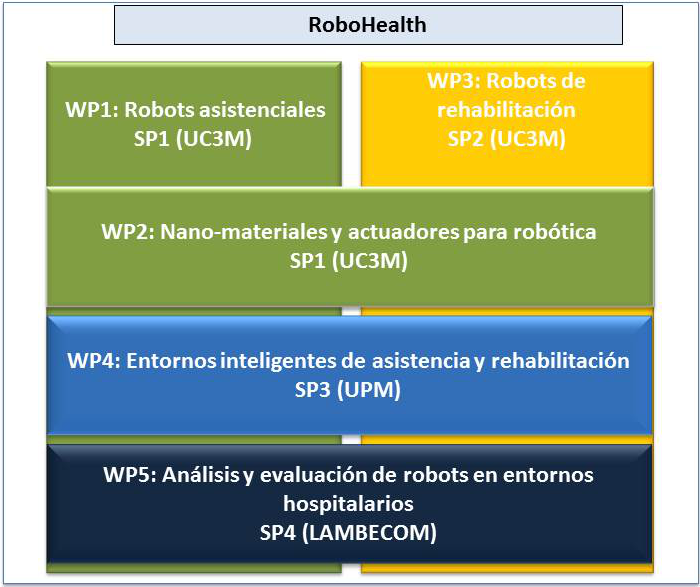
\includegraphics[width=0.55\textwidth]{figuras/RHstruct.png}
\caption{Estructura RoboHealth}
\label{fig:RH}
\end{figure}

Dentro del marco previamente expuesto, se han desarrollado dos plataformas que sirven de base para el proyecto objetivo de este documento.

\begin{itemize}
\item \textbf{RoboHealth Arm} es un brazo robótico de tres grados de libertad (actualmente, cuenta con sólo dos grados de libertad operativos) diseñado para sustentar una tablet en su extremo, haciendo más acesible su uso para pacientes y cuidadores. Está basado en un sitema de cuerdas y poleas accionado por tres servomotores.
\item Por otro lado, existe una aplicacion de \textbf{Node-RED} que integra los diferentes dispositivos y proyectos desarrollados en una red domótica. Incluye una interfaz gráfica que facilita su interacción vía internet, posibilitando controlar los dispositivos desde cualquier lugar.
\end{itemize} 

La idea es continuar el proceso de integración de los diferentes dispositivos en Node-RED con la intención de controlar todo desde la misma interfaz. En ese contexto, surge el proyecto de hacerlo con el brazo RoboHealth Arm. Con el fin de tratar de explorar todas las tecnologías posibles, se comprueba que la radiofrecuencia aún no habia sido y existen soluciones económicas en el mercado.

Así, el planteamient del Trabajo Final de Grado tomó forma, defiendose como la conexión mediante el uso de radiofrecuencia del brazo RoboHealth Arm a la interfaz de Node-RED. Para la radiofrecuencia, se usarán dispositivos XBee.

\section{Objetivos}

El fin del proyecto es la completa integración de un control a través de internet del brazo robótico. Los comandos se lanzan desde la interfaz de Node-Red y el ordenador de la sala transmite la orden vía radiofrecuencia al brazo.

Se ha desarrollado a posibilidad de configurar las coordenadas articulares del brazo antes de ser enviadas, dentro de su rango óptimo de trabajo actual.

La orden de Node-Red pone en marcha la ejecución de un script en Python que toma esos parámetros previamente especificados y envía por uno de los puertos serie el correspondiente frame. Este frame está pensado de acuerdo a las especificaciones de comunicación del brazo y del encapsulamiento de las comunicaciones de radio.

Un dispositivo XBee ha sido configurado para enviar el frame de datos recibido por comunicación serial. Al poder concentrarse todo el procesamiento de la información correspondiente al emisor en el anteriormente mencionado script, no se precisa de ningún microcontrolador adicional que funcione junto al módulo de radiofrecuencia. Así pues, el módulo XBee funciona de manera exclusiva como un traductor entre la información en el puerto serie correspondiente y las ondas de radiofrecuencia.

El dispositivo XBee receptor de la información que comanda el brazo robótico esta situado en el mismo. Su objetivo es ser capaz de captar el mensaje de radio específicamente diseñado para él y transmitirlo al microcontrolador del brazo. De la misma manera que en el otro XBee, su función será la de traductor de las ondas de radio (excusivamente de las destinadas a él) en información en el puerto serial. Esto es posible gracias al prediseño de los frames de información de acuerdo a las especificaciones y protocolos de comunicación del brazo.

El dispositivo operativo provoca la reacción esperada en el brazo, moviendo sus servos hasta las coordenadas articulares especificadas.

\section{Materiales utilizados}

Aquí se pueden citar todos los materiales utilizados, tanto software como hardware, para que el lector tenga una primera de lo que se va a hablar en el TFG.

\subsection{Componentes hardware}

\subsection{Componentes software}

\section{Estructura del documento}

A continuación y para facilitar la lectura del documento, se detalla el contenido de cada capítulo.

\begin{itemize}
\item En el capítulo 1 se realiza una introducción.
\item En el capítulo 2 se hace un repaso...
\end{itemize}

  
%partes finales del trabajo: conclusiones, bibliografia y anexos

\chapter{Marco Teórico}

En este capítulo se describen (brevemente) todos los conceptos necesarios para entender el trabajo. No se trata de copiar el contenido de los libros de texto, si no de hacer un resumen de los conceptos necesarios para facilitar la lectura del documento al lector. Se entiende que el lector de un TFG tiene que tener unos conocimientos mínimos sobre el tema.
  
\chapter{Estado del arte}

A continuación, se hace un repaso de la tecnología existente en la actualidad relacionada con los campos tocados por el presente proyecto. El objetivo es proporcionar al lector un punto de partida del trabajo y comentar las soluciones utilizadas por otros autores. 

\section{Water level control using Raspberry Pi + XBee + XBMQ + MQTT + Node-Red \cite{zhivazhiva:RaspberryPi}}

Se trata de un proyecto que trabaja de manera bastante similar al trabajo objetivo del presente documento, teniendo ciertas tecnologías en común.

El objetivo es el control de una pequeña bomba de agua que llena un depósito lentamente, con una distancia considerable entre ambos elementos y el ordenador central. La motivación para automatizar el proceso de llenado del depósito era evitar ciertos incidentes provocados por el olvido de la persona que controlaba la bomba, debido a los extensos tiempos que se tomaba el sistema para llenar el depósito. El autor comenta que la señal se perdía frecuentemente al usar unos módulos Wi-Fi baratos y terminó decidiéndose por la tecnología XBee de Digi, descartando cualquier tecnología que no fuera inalámbrica por los motivos de distancia comentados previamente.

\begin{figure}[tb]
\centering
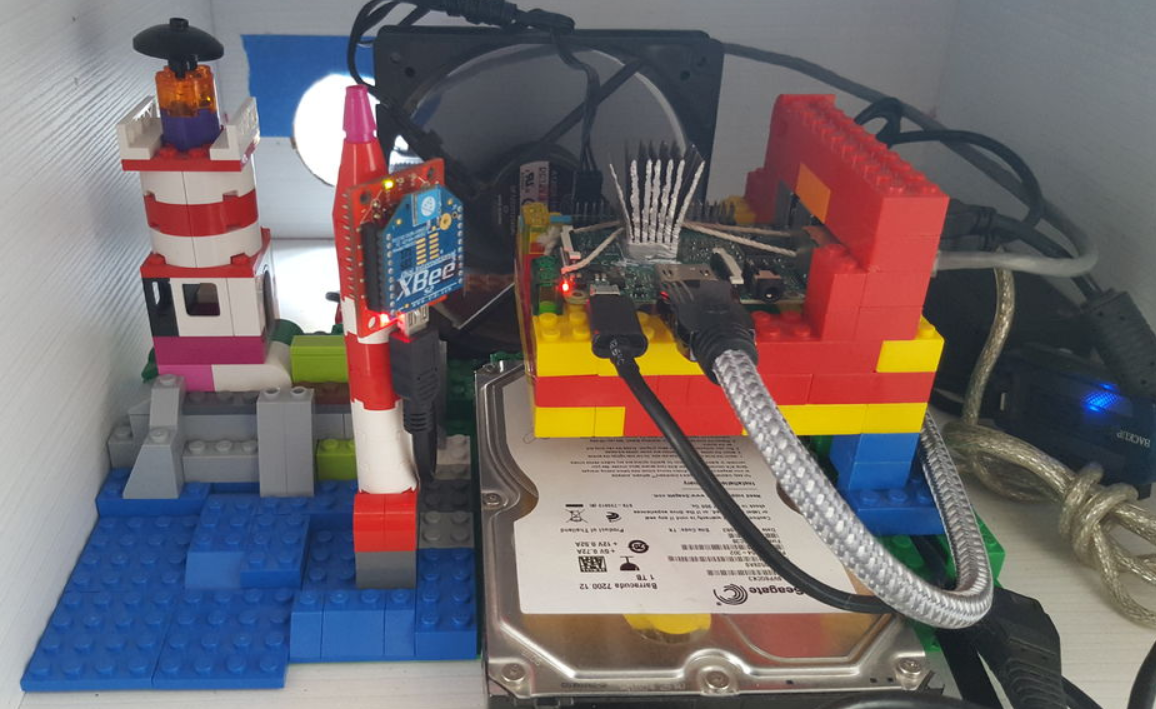
\includegraphics[width=0.55\textwidth]{figuras/EArte1.png}
\caption{Montaje del proyecto 3.1}
\label{fig:EArte1}
\end{figure}

Una Raspberry Pi3 ejerce de ordenador central del sistema y es el componente encargado de coordinar la interacción con el usuario que manda la orden y la interacción con el depósito y la bomba de agua vía XBee (montaje en la figura \ref{fig:EArte1}).

\begin{itemize}
\item Por un lado, tiene instalado Mosquitto (MQTT); un programa que usa la red para crear una especie de "tablón de anuncios" virtual. Los dispositivos conectados a esa red pueden suscribirse a un \textit{topic} y recibir lo que otros dispositivos publican en él.
La idea es que, haciendo uso de diferentes aplicaciones (como puede ser el caso de \textit{IoT MQTT Dashboard} en Android), se puedan publicar ciertos mensajes en algún \textit{topic} al que esté suscrita la Raspberry Pi desde otros dispositivos de manera remota. La Raspberry recibe esta información y actúa en consecuencia.
\item XBMQ actúa de puente dentro de la Raspberry Pi entre MQTT y el módulo XBee conectado a la misma, que es el que se comunica con el actuador y el sensor.
\item La Raspberry Pi envía los comandos al actuador y recibe la información del sensor a través del módulo XBee. En el lado del depósito, se sitúa el otro XBee con una salida controlando un pequeño relé que acciona y desactiva la bomba y una entrada que envía al XBee de la Raspberry el estado del sensor. Huelga mencionar que ambos XBee se han debido configurar adecuadamente.
\item Para detener la bomba si el sensor detecta que el depósito está lleno, se precisa de cierta lógica que se programa en la Raspberry usando otra tecnología que se verá mas en detalle: Node-Red. El uso de este programa permite automatizar otras acciones paralelas como, por ejemplo, publicar un tweet cada vez que la bomba cambie de estado.
\end{itemize}

\section{Servidor Raspberry Pi-XBee en Python \cite{JONIUZ:IoT}}

El proyecto detalla la conexión de un Arduino Uno y una Raspberry Pi a través de XBee. Viene siendo algo muy similar a una de las etapas del trabajo detallado en este documento.

En el lado del Arduino Uno, emplea una XBee Shield 2.0 de Sheeed Studio (figura \ref{fig:EArte2}) para implemental el módulo de radio frecuencia.

\begin{figure}[tb]
\centering
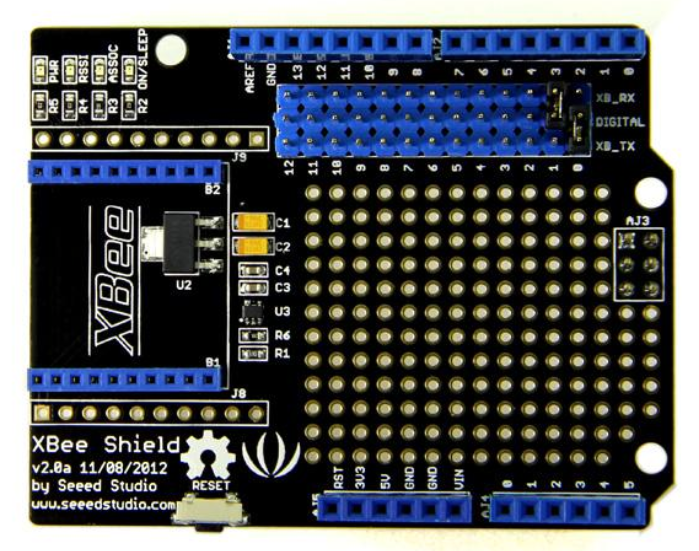
\includegraphics[width=0.55\textwidth]{figuras/EArte2.png}
\caption{XBee Shield v2.0 - Seeed Studio}
\label{fig:EArte2}
\end{figure}

Si se habla del lado de la Raspberry Pi, la interacción con el módulo XBee se realiza a través de una placa XBee Explorer.

Como uno puede comprobar, existe una gran variedad de placas y shields que adaptan y facilitan la interacción de los módulos XBee con las plataformas de ordenadores y microcontroladores más populares.

En este caso, los módulos XBee están configurados como AT. Más adelante en el documento se detalla esta cualidad.

\section{Smart Porch Light Project \cite{SPLP:MOUSER}}

En el contexto del Internet de las Cosas (IoT), el autor desarrolla un proyecto de red inalámbrica de sensores y actuadores sincronizados a una nube en la red.

El caso particular consta de una luz de exterior que es automáticamente controlada teniendo en cuenta los datos obtenidos de múltiples sensores que captan el estado del entorno. Estos sensores miden la luz ambiente, temperatura, humedad y luz ultravioleta. El control de la lámpara de exterior se lleva a cabo con un relé capaz de separar la etapa de potencia de la etapa de señal. Con el proyecto operativo, se usan servicios en la nube para almacenar y leer la información del estado del sistema; obteniendo como resultado una lámpara inteligente que permite mostrar a los usuarios el estado de los sensores desde cualquier dispositivo con acceso a internet.

Los componentes hardware, al ser todos del mismo fabricante (Seeed Studio), permiten su apilamento en un único stack compacto (figura \ref{fig:EArte4}) de microcontrolador, shields módulo XBee. El microcontrolador es un Arduino Mega, los shields son de sensores y de XBee y,coronando el stack, se encuentra el módulo XBee LTE.

\begin{figure}[t]
\centering
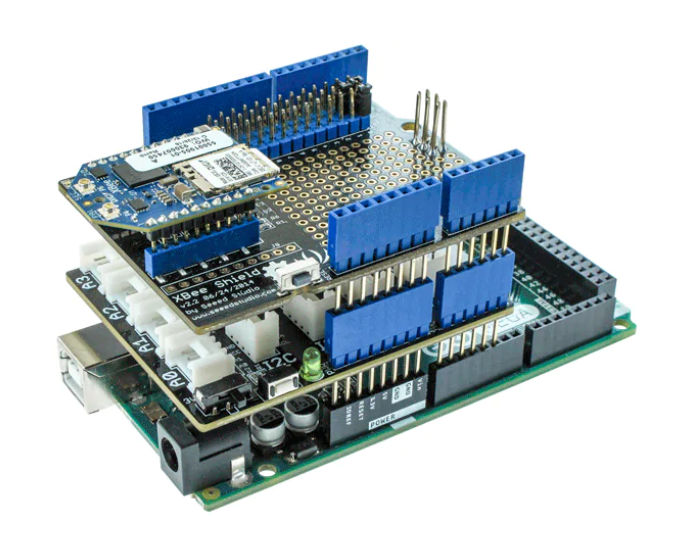
\includegraphics[width=0.55\textwidth]{figuras/EArte4.png}
\caption{Stack Hardware del proyecto 3.4}
\label{fig:EArte4}
\end{figure}

A diferencia de proyectos mencionados anteriormente, en este se usa una API REST en lugar de MQTT para transferir la información al servicio de nube correspondiente y los módulos XBee son del modelo LTE, por lo que pueden acceder a la red directamente sin la necesidad de poseer enlace alguno a un ordenador con conexión, bien vía USB o a través de otro módulo XBee. Por otro lado, la interfaz donde mostrar el estado de los sensores no se basa en Node-RED, sino en Ubidots.

\section{Home Automation System \cite{Molnar:Digi}}

Estamos ante otro proyecto del campo IoT que hace uso de módulos XBee. En este caso, los actuadores y sensores de una casa en la que se ha implementado este sistema domótico están conectados a red inalámbrica de módulos XBee mediante cableados como el que se muestra en la figura \ref{fig:EArte5}.

\begin{figure}[tb]
\centering
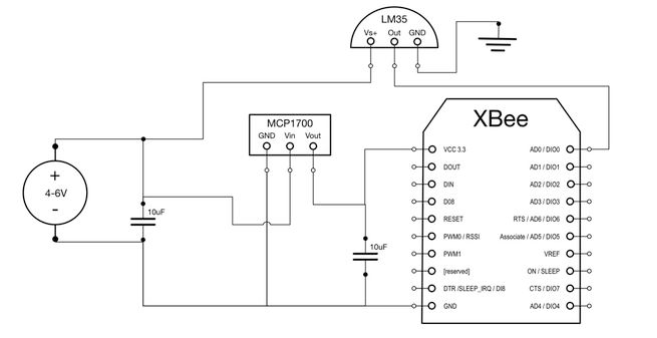
\includegraphics[width=0.55\textwidth]{figuras/EArte5.png}
\caption{Esquema de conexión del sensor de temperatura}
\label{fig:EArte5}
\end{figure}

La información se transmite a un portal central que tiene como base una placa Netduino o una Raspberry Pi con Windows IoT como sistema operativo. El portal envía y recibe mensajes de cada uno de los módulos XBee conectados y traduce la información de tal manera que el controlador lo pueda interpretar.

Usa MQTT para la comunicación controlador-portal pero recurre a una nueva herramienta, openHAB, para proporcionar una interfaz gráfica donde monitorizar y controlar los sensores y actuadores de la casa.

\section{Controlador central para un sistema domótico utilizando el protocolo inalámbrico ZigBee \cite{ULL:2016}}

Con este proyecto se habla del desarrollo de otro sistema domótico; esta vez basado en la placa de desarrollo Pandaboard (figura \ref{fig:EArte6}). A principios de la presente década, Pandaboard nació para competir en el mercado de los ordenadores pequeños de bajo coste, pero Raspberry terminó por dominar a la competencia. Hoy en día se trata de una placa obsoleta y poco usada por la comunidad.

\begin{figure}[tb]
\centering
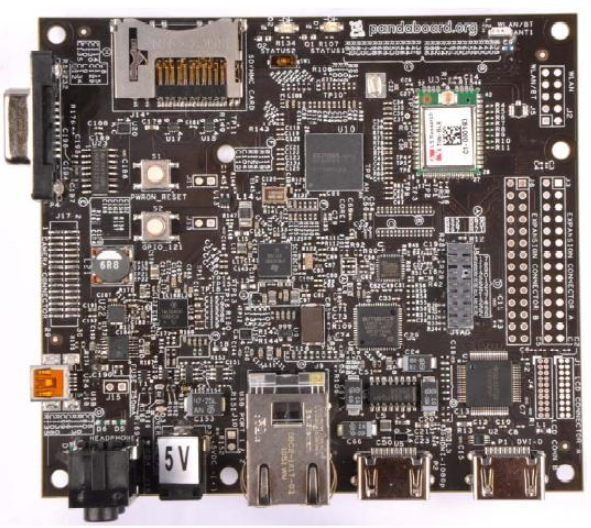
\includegraphics[width=0.55\textwidth]{figuras/EArte6.png}
\caption{PandaBoard ES}
\label{fig:EArte6}
\end{figure}

En este proyecto se recurre también al uso de dispositivos XBee para la transmisión de información y a MQTT. Incorpora Domoticz, un programa de supervisión y configuración domótica de código abierto.

Como particularidad de la que se hablará de manera mas detallada más adelante, en este caso los módulos XBee funcionan en configuración API, en contraposición al modo AT mencionado previamente en otro proyecto.

\section{Node-RED based custom full-room wake-up light \cite{Bulten:2019}}

Proyecto que desarrolla una aplicación Node-RED con el fin de configurar un patrón despertador configurable. El desarrollo del proyecto referenciado \cite{Bulten:2019} se centra en la definición de los flujos de Node-RED puesto que el sistema domótico se ha desarrollado previamente \cite{Bulten:2018}.

El flujo de Node-RED (figura \ref{fig:EArte7}) trabaja detectando la igualdad entre la hora programada y la actual. A continuación, comprueba si es fin de seamana y si está activada la alarma durante los fines de semana en la configuración. Por último y habiendo superado las etapas anteriores, se define una secuencia de iluminación de las bombillas correspondiente a la señal de despertador.

\begin{figure}[tb]
\centering
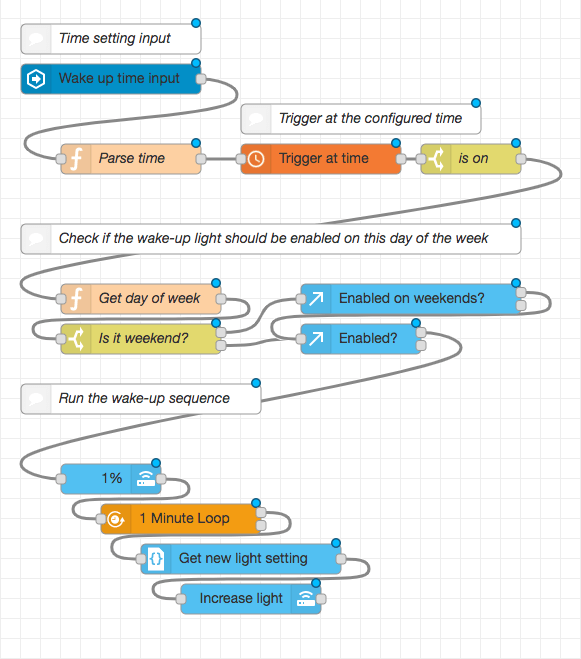
\includegraphics[width=0.75\textwidth]{figuras/EArte7.png}
\caption{Flujo de Node-RED}
\label{fig:EArte7}
\end{figure}

El proyecto domótico completo se basa en una instalación de Node-RED y Home Assistant, que proporciona la interfaz de usuario, sobre una Raspberry Pi. Las bombillas son bombillas inteligentes que reciben ordenes vía XBee. La recepción y envío de radiofrecuencia desde la Raspberry Pi se produce a través de un hub comercial que va alternando la conexión con las diferentes bombillas a muy alta velocidad.

\section{ArduSmartHome \cite{UOC:2017}}

El proyecto ArduSmartHome consiste en el desarrollo de un sistema domótico de control que capture datos del entorno a través de varios sensores y monitorizar esa información usando Node-RED.

La principal diferencia que tiene este proyecto con los mencionados previamente es la tecnología usada para la transmisión de la información. Mientras que hasta ahora se habiía usado principalmente radiofrecuencia a través de módulos XBee\footnote{La tecnología utilizada en el proyecto que describe este documento es, precisamente, radiofrecuencia usando módulos XBee}, en este caso se usa una red WiFi local.

\begin{figure}[tb]
\centering
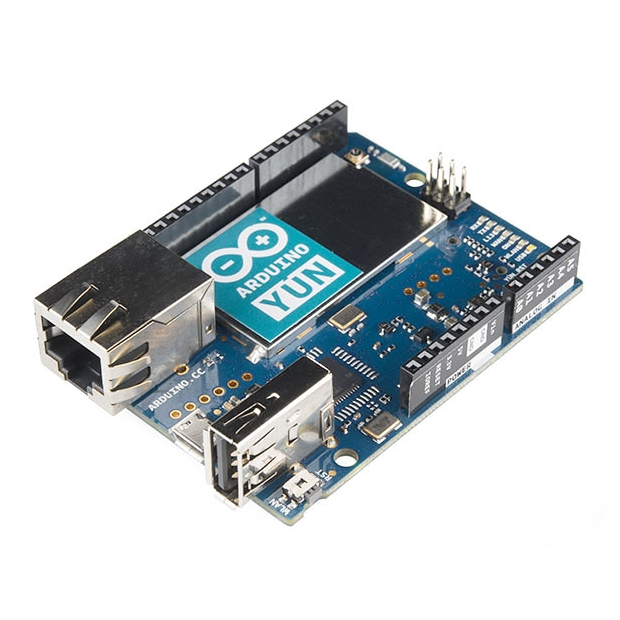
\includegraphics[width=0.55\textwidth]{figuras/EArte8.png}
\caption{Arduino Yun}
\label{fig:EArte8}
\end{figure}

Para conseguir esto, se hace uso de un microcontrolador diseñado para esta tarea, el Arduino Yun (figura \ref{fig:EArte8}). La red domótica posee varios de estos microcontroladores volcando los datos de los sensores que tienen conectados a la red local. Existe un Arduino Yun\footnote{Se puede lograr una equivalencia económica al Arduino Yun usando un Arduino UNO complementado con la shield de extensión Dragino Yun Shield v2.4} que ejerce las funciones de coordinador de las comunicaciones a la vez que es quién se encarga de establecerlas. En este proyecto también se hace uso de MQTT.

\section{University of Minnesota – Solar Vehicle \cite{UM:SV}}

Estudiantes de la Universidad de Minnesota llevan desde 1990 desarrollado prototipos de coches solares para competir en varios certámenes a nivel nacional e internacional, obteniendo grandes resultados. En este contexto, en 2019 se ha presentado el nuevo prototipo denominado EOS II (figura \ref{fig:EArte3}). 

\begin{figure}[b]
\centering
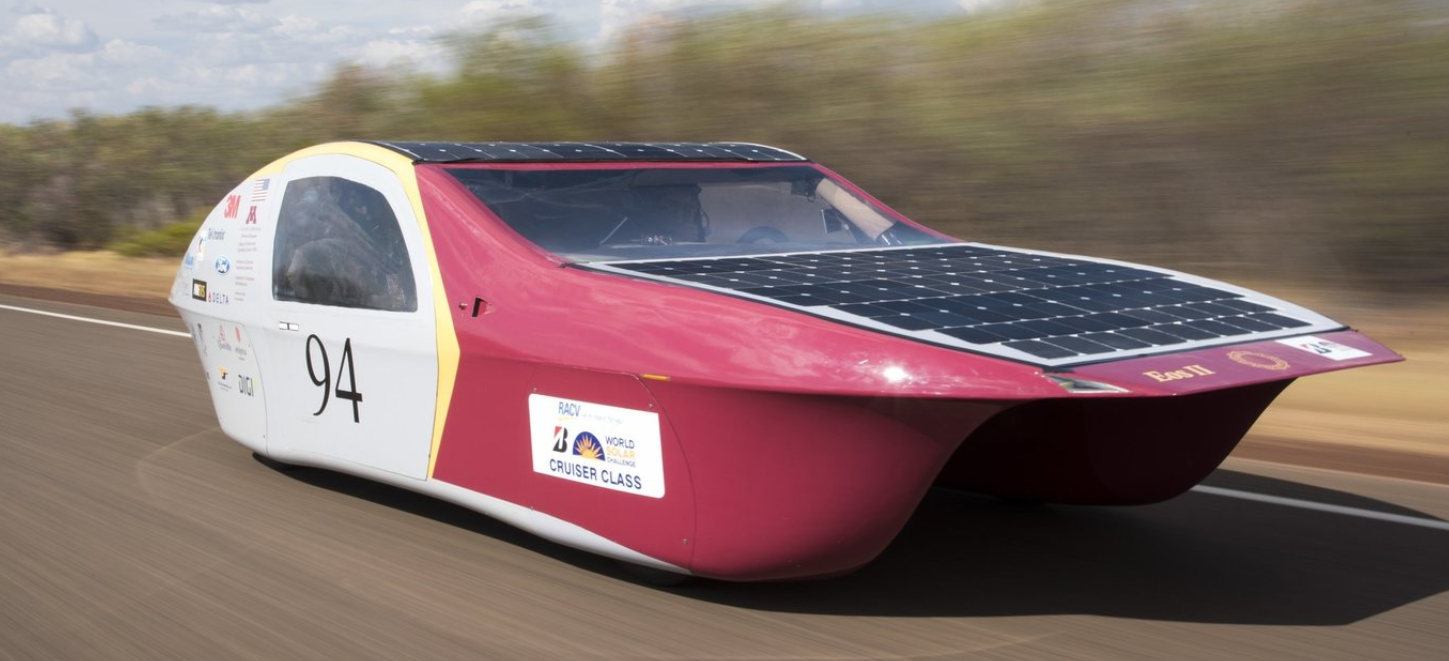
\includegraphics[width=0.55\textwidth]{figuras/EArte3.png}
\caption{EOS II Solar car}
\label{fig:EArte3}
\end{figure}

Con el apoyo de Digi, han implementado una red inalámbrica a la que conectan ordenadores y diferentes sensores. La conexión a esta red se realiza mediante módulos XBee. El objetivo final es la comunicación entre los módulos para la detección de errores y el almacenamiento de los datos adquiridos por esos mismos sensores durante el funcionamiento del prototipo.

\definecolor{verde_p}{rgb}{0.77,0.97,0.84}
\definecolor{amarillo_claro}{rgb}{1,1,0.90}

\chapter{Diseño del proyecto}

\section{Planteamiento inicial}

El desarrollo se ha llevado a cabo de manera modular. Se ha planteado el trabajo en bloques individuales para terminar comunicándolos por su respectiva vía.

Los objetivos descritos en la sección \ref{sec:refobj} sirven de guía para definir responsabilidades de cada módulo.

En la figura \ref{fig:diainteraccion} se puede observar el diagrama de interacciones entre los diferentes módulos

\begin{figure}[tb]
\centering
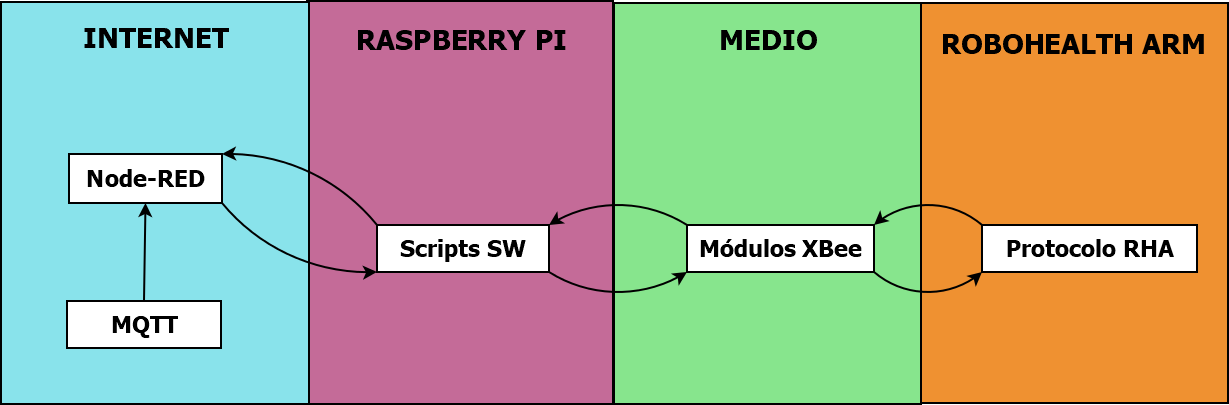
\includegraphics[width=1\textwidth]{figuras/DiaInteraccion.png}
\caption{Diagrama de interacción}
\label{fig:diainteraccion}
\end{figure}

Se establece una comunicación bidireccional en la que, por un lado, se envían comandos desde varias fuentes de mando y, por el otro, se reciben los mensajes periódicos de estado que envía el RoboHealth Arm.

Las fuentes de mando se emplazan en la red, desde donde se interactúa con el usuario. Una de ellas es Node-RED, la base de la red domótica y la otra es Mosquitto (MQTT), que diversifica el tipo de dispositivos desde los que se puede interactuar con el brazo.

La Raspberry Pi es el punto donde las órdenes enviadas desde la red toman forma en una salida serial.

Los módulos XBee se encargan de la transmisión inalámbrica de la información a través del medio\footnote{En la sección \ref{sec:radiofrec} se detalla el proceso del envío de ondas electromagnéticas a través del aire}.

Esta información es captada por el brazo robótico de acuerdo a un protocolo de comunicación prediseñado y actúa en consecuencia.

Haciendo una analogía con los diagramas de casos de uso propios del Lenguaje de Modelado Unificado (UML) en el campo del desarrollo software, a continuación (figura \ref{fig:diacasos}) se analizan las distintas acciones que puede efectuar el usuario y cómo debería reaccionar el sistema ante estas acciones. Nótese que se ha tomado al brazo robótico como un actor más dentro del sistema domótico.

\begin{figure}[tb]
\centering
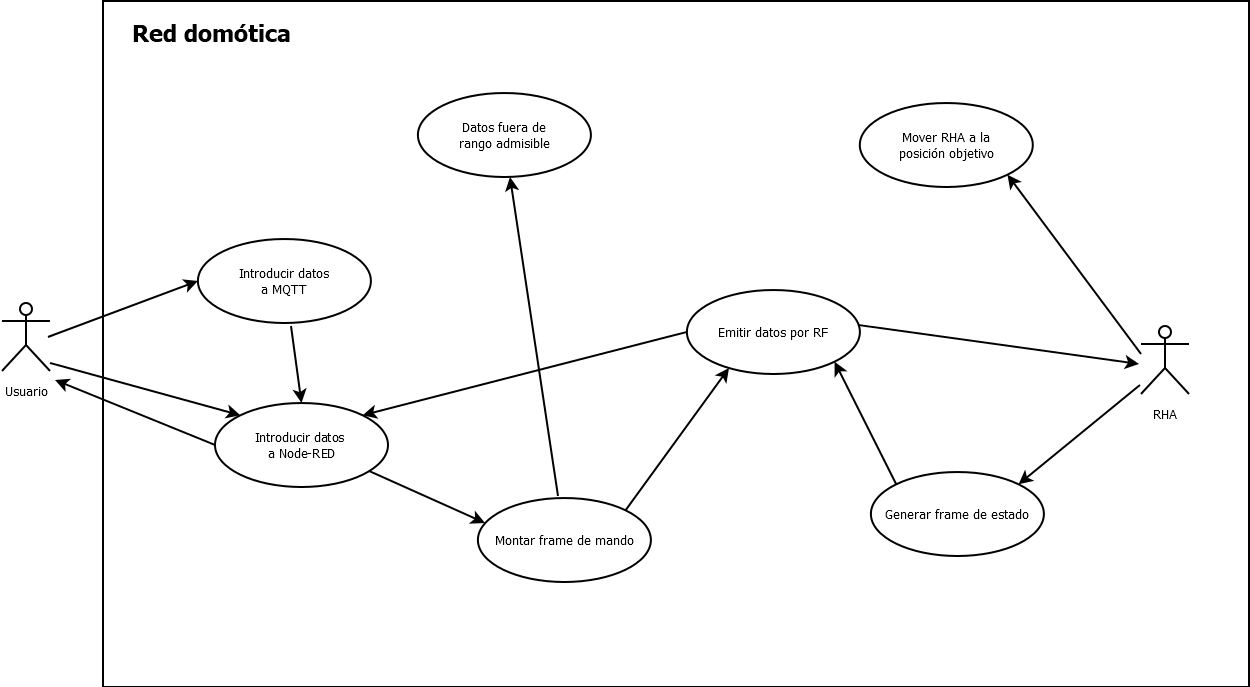
\includegraphics[width=1\textwidth]{figuras/DiaCasos.png}
\caption{Diagrama de casos de uso}
\label{fig:diacasos}
\end{figure}

Continuando con el uso de conceptos UML, en la imagen \ref{fig:diasecuencia} se puede observar la secuencia de acciones planificadas para el envío de información al brazo robótico.

\begin{figure}[tb]
\centering
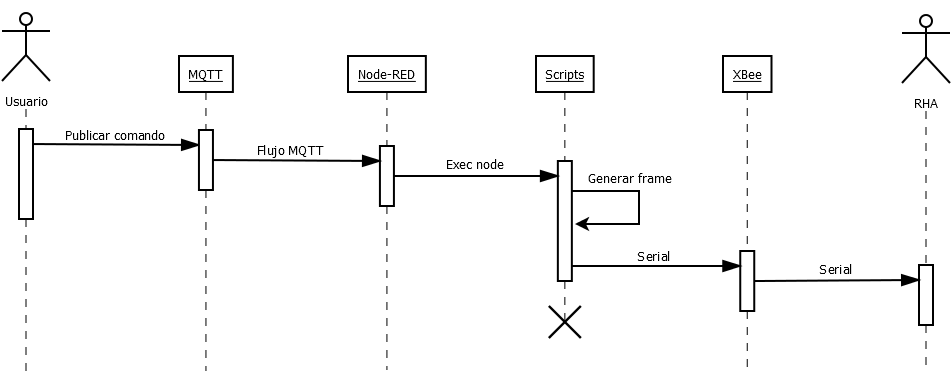
\includegraphics[width=1\textwidth]{figuras/DiaSecuencia.png}
\caption{Diagrama de Secuencia de envío}
\label{fig:diasecuencia}
\end{figure}

Con los objetivos y conceptos establecidos, se puede pasar al desarrollo siguiendo una metodología modular, como se ha indicado antes.

\section{Unidad de mando}

La base de las comunicaciones debe ser un ordenador. Las funciones de este ordenador o unidad de mando pasan por la coordinación de los diferentes elementos de la red domótica, incluyendo tanto el control de estos como la recepción de sus estados.

Es posible (y deseable) que ciertos elementos tengan otro control independiente a la red domótica. Así, por ejemplo, una persiana conectada a la red domótica podría ser accionada por el mismo ordenador sin obviar que el mecanismo podría accionarse a través de un pulsador. Esto hace necesaria la monitorización de la mayor parte posible de elementos. Podría darse el caso de que, incluso, la acción de ciertos elementos fuera mecánica en complementación a la acción de naturaleza electrica, imposibilitando cualquier integración de estos métodos alternativos de accionamiento en la red domótica. 

La unidad de mando debe encargarse de igual manera de la interacción con el usuario, aportando una interfaz.

Los requisitos de un sistema domótico no son especialmente exigentes en cuanto a la capacidad de procesamiento, por lo que características como un tamaño contenido o un bajo coste se valoran positivamente en la elección del ordenador0
.
En este contexto, se hace uso de la popular Raspberry Pi 3 Model B (figura \ref{fig:RPi3}) para el cometido descrito.

\subsection{Rasberry Pi 3 Model B}

La Raspberry Pi 3 Model B es uno de los más actuales modelos\footnote{Sólo se encuentra la Raspberry Pi 3 Model B+ con una fecha de lanzamiento posterior} de la tercera generación de este popular micro-ordenador de bajo coste. Si se miran sus especificaciones, se puede observar que, corriendo a través de una CPU Broadcom BCM2837 de 64 bits a 1.2GHz, posee:

\begin{itemize}
\item 1GB de memoria RAM
\item Conexión LAN inalámbrica y módulo Bluetooth integrados
\item Puerto Ethernet
\item 40 pines de entrada/salida (GPIO)
\item 4 puertos USB 2.0
\item Salida stereo de 4 polos
\item Conector HDMI
\item Puerto de cámara CSI
\item Puerto de display DSI
\item Puerto microSD
\item Puerto microUSB
\end{itemize}

Se puede observar el layout de estos componentes sobre la placa en la figura \ref{fig:RPilayout}.

\begin{figure}[tb]
\centering
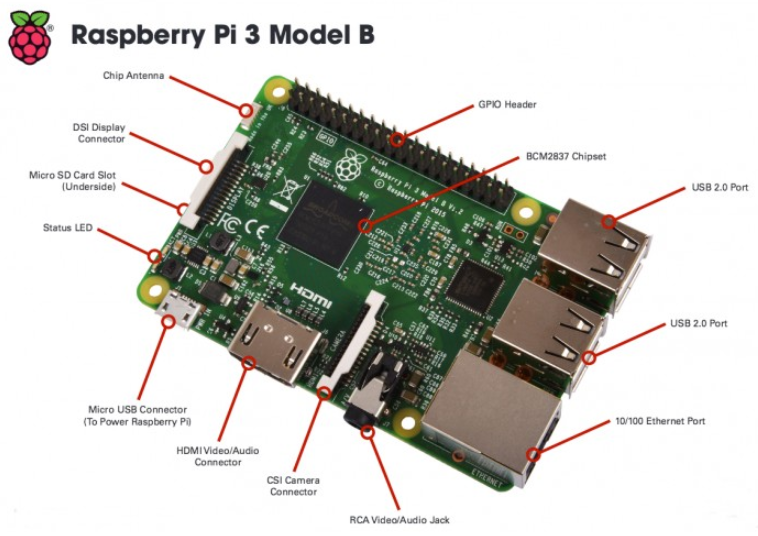
\includegraphics[width=0.75\textwidth]{figuras/RPiLayout.png}
\caption{Layout de puertos de la Raspberry Pi}
\label{fig:RPilayout}
\end{figure}

El puerto microUSB tiene la función de alimentar al ordenador. Se debe conectar una alimentación de 5 voltios a 2.5 amperios. Podría funcionar con una fuente de menos potencia pero podría ser que no soportara la inclusión de ciertos periféricos.

El puerto microSD sirve de alojamiento para la memoria ROM de la Raspberry. A través de este puerto, se carga el sistema operativo y se utiliza la memoria libre como almacenamiento interno.

\subsubsection{Raspbian OS}

Raspbian OS es el sistema operativo utilizado en la Raspberry Pi del laboratorio (figura \ref{fig:raspbian}). Se trata de una distribución no oficial basada en Debian adaptada a las especificaciones de la placa computadora Raspberry Pi. Debian está basado en el sistema GNU/Linux y, por tanto, se habla de software libre. El software, con sus características y actualizaciones, es desarrollado por la comunidad.

\begin{figure}[tb]
\centering
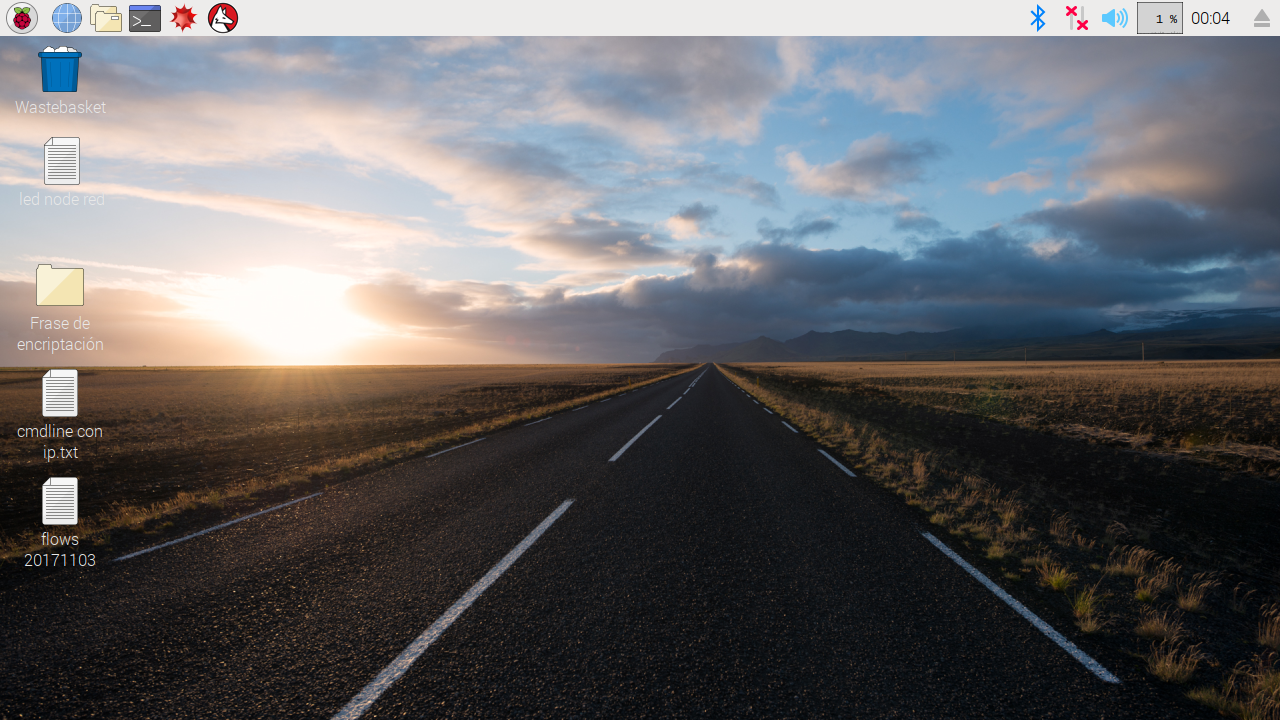
\includegraphics[width=0.7\textwidth]{figuras/Raspbian.png}
\caption{Escritorio de Raspbian}
\label{fig:raspbian}
\end{figure}

Entre otras funcionalidades, destaca el poder configurar la Raspberry de manera sencilla a través del menú \textit{raspy-config}

En el Anexo \ref{anexo:raspbian} se encuentran las instrucciones para obtener Raspbian 9.1 (Stretch) instalado en la Raspberry. Esta es la última distribución estable a día de hoy.

\subsubsection{Comunicación con otros ordenadores}

% Configuración de la visualización del código SW
\lstset{backgroundcolor=\color{verde_p}, language=bash, breaklines=true, basicstyle=\footnotesize, xleftmargin=25pt, framesep=8pt, numbersep=15pt}

A la hora de trabajar con la Raspberry instalada, no es usual que sea deseable la instalación de periféricos de entrada y salida para interactuar con ella. Es por esto por lo que se recurre a una conexión SSH para trabajar desde remoto con otro ordenador exactamente de igual manera a la que lo haríamos desde la ventana de comandos de Linux.

El procedimiento es diferente en función de si la conexión se efectúa desde una máquina en Linux o en Windows

\begin{itemize}
\item \textbf{Conexión SSH desde Windows}

En Windows existen varios programas dedicados a establecer conexiones entre dispositivos. Uno de los más conocidos es \textbf{Putty} (figura \ref{fig:putty}), en cuya interfaz puedes introducir la dirección IP del cliente\footnote{La dirección IP de la Raspberry Pi se puede obtener usando el comando \textit{ifconfig} una vez la conexión a internet ya ha sido establecida}, un puerto libre y el tipo de conexión que deseas (SSH, en nuestro caso). Al pulsar \textit{Open} se abre un terminal en el que se solicitan las credenciales antes de tener acceso completo a la Raspberry.

\begin{figure}[H]
\centering
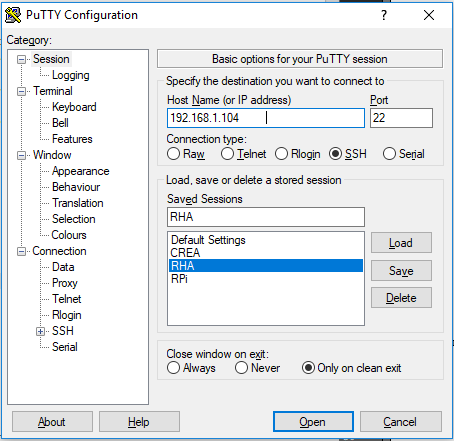
\includegraphics[width=0.5\textwidth]{figuras/Putty.png}
\caption{Interfaz de Putty}
\label{fig:putty}
\end{figure}

\item \textbf{Conexión SSH desde Linux}

En Linux se puede establecer una conexión SSH haciendo uso del terminal

\begin{lstlisting}[frame=single, label=command:ssh]
$ ssh root@190.168.1.104
\end{lstlisting}

El comando \textit{ssh} establece este tipo de conexiones. El usuario se indica en el lugar de \textit{root} en el ejemplo mientras que la IP del remoto se sitúa después del arroba. Es posible configurar el puerto con la opción \textit{-p} (por defecto se usa el puerto 22).

\begin{lstlisting}[frame=single, label=command:ssh-p]
$ ssh -p 22 root@190.168.1.104
\end{lstlisting}

De igual manera que en Windows, se solicitará la contraseña del usuario si procede y se accederá al terminal.

\end{itemize}

\subsection{MQTT}

Mosquitto (Message Queue Telemetry Transport) es un protocolo de código abierto enfocado a las conexiones Machine-to-Machine (M2M) \cite{Vega:2016} que se ha popularizado entre diferentes aplicaciones que precisan de comunicación entre sensores y mandos de redes domóticas. Entre sus características se encuentra un consumo de recursos muy bajo.

Su funcionamiento se basa en una configuración de estrella. Trabaja con un nodo central (también llamado Broker) con el que se establecen conexiones bidireccionales desde múltiples clientes (figura \ref{fig:mqtt}). Estas conexiones son cifradas, aportando una capa de seguridad a la red domótica.

\begin{figure}[tb]
\centering
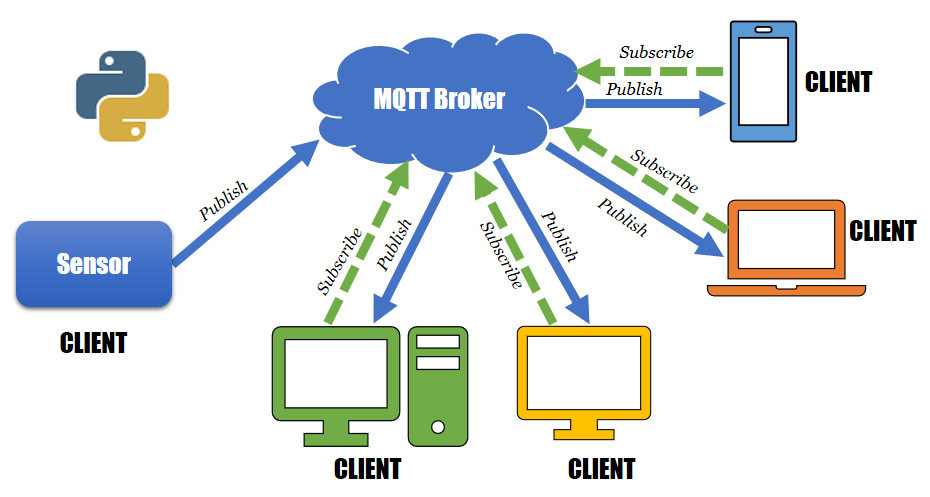
\includegraphics[width=0.75\textwidth]{figuras/mqtt.png}
\caption{Arquitectura MQTT}
\label{fig:mqtt}
\end{figure}

El concepto de \textit{topic} es la forma que tiene MQTT de articular las comunicaciones. Se puede hacer una analogía de los \textit{topic} con un tablón de anuncios. La gente puede publicar en el tablón lo que le plazca y esto será visto por aquellos que se paren a mirar el tablón. De igual manera funciona MQTT, cualquier cliente puede publicar en un \textit{topic} y este mensaje será recibido por aquellos clientes que estén suscritos a ese mismo \textit{topic}. Los \textit{topics}, además, son jerarquizables. Esto es, pueden generarse subtopics de manera recurrente con el fin de poder enviar mensajes únicamente a un grupo de clientes si se observa la red desde una perspectiva más global.

Existen varios \textit{Broker} de MQTT pero, con diferencia, el más popular es el llamado Mosquitto.

Una guía para su instalación puede encontrarse en el Anexo \ref{anexo:mqtt}

\subsubsection{MQTT en RoboHealth}\label{subsubsec:RH_MQTT}

En cuanto al funcionamiento dentro de la habitación, existe un topic denominado \textit{Robohealth/room/devices} donde publican los distintos dispositivos mientras Node-RED está suscrito.

Los mensajes en el topic de la habitación siguen un mismo formato:

$$\{'id':xx,'atrib1':'yy','atrib2':'zz',(...)\}$$

\textit{xx} remplaza el identificador del cliente, único para cada dispositivo. RoboHealth Arm ha sido identificado con el número \textbf{99}.

\textit{atrib1}, \textit{atrib2} y sucesivos son atributos a los que se les quiere dar un valor. En el caso de los dispositivos digitales el atributo suele ser único, siendo denominado \textit{status}. En el caso de RoboHealth Arm es posible trasladarle dos atributos correspondientes a las coordenadas articulares objetivo del robot. Los atributos son \textbf{shoulder} para el hombro y \textbf{elbow} para el codo.

\textit{yy}, \textit{zz} y sucesivos son los valores correspondientes a los atributos. En el caso del brazo deberán pasarse las dos \textbf{coordenadas articulares en formato hexadecimal}.

\subsection{Node-RED}\label{subsec:nodered}

Node-RED es una herramienta de programación basada en una interfaz de programación online representada a través de flujos y nodos (figura \ref{fig:nodeinterfaz}). Viene preinstalada en Raspbian Stretch, lo que puede dar una idea del grado de integración que tiene esta herramienta en la comunidad.

Los flujos representan caminos de transmisión de los objetos de node-RED, denominados por defecto \textit{msg}. Estos objetos \textit{msg} poseen unos atributos, algunos creados por defecto y otros opcionales customizados. Uno de los atributos por defecto es \textit{payload}, que suele ser utilizado como contenedor de la información a trasladar. Esta información puede ser de casi cualquier tipo, desde un booleano hasta otro objeto con sus propios atributos. El otro de los atributos por defecto es \textit{\_msgid}, que es un identificador del mensaje enviado que sirve para monitorizar su estado a lo largo del flujo.

Los nodos son etapas en las que, basándose en diferentes tecnologías, se realiza una acción cuando se produce la entrada del mensaje a través del flujo. Esta acción puede ir desde producir algún tipo de reacción ajena a Node-RED hasta modificar variables internas del programa, modificando (o no) el mensaje de flujo antes de volver a transmitirlo.

Existen nodos relacionados con un gran número de tareas. La comunidad puede aportar sus propios paquetes de nodos, ampliando progresivamente el número de tecnologías compatibles con Node-RED. Algunos de los nodos más representativos y usados en el proyecto Robohealth son los siguientes:

\begin{figure}[H]
\centering
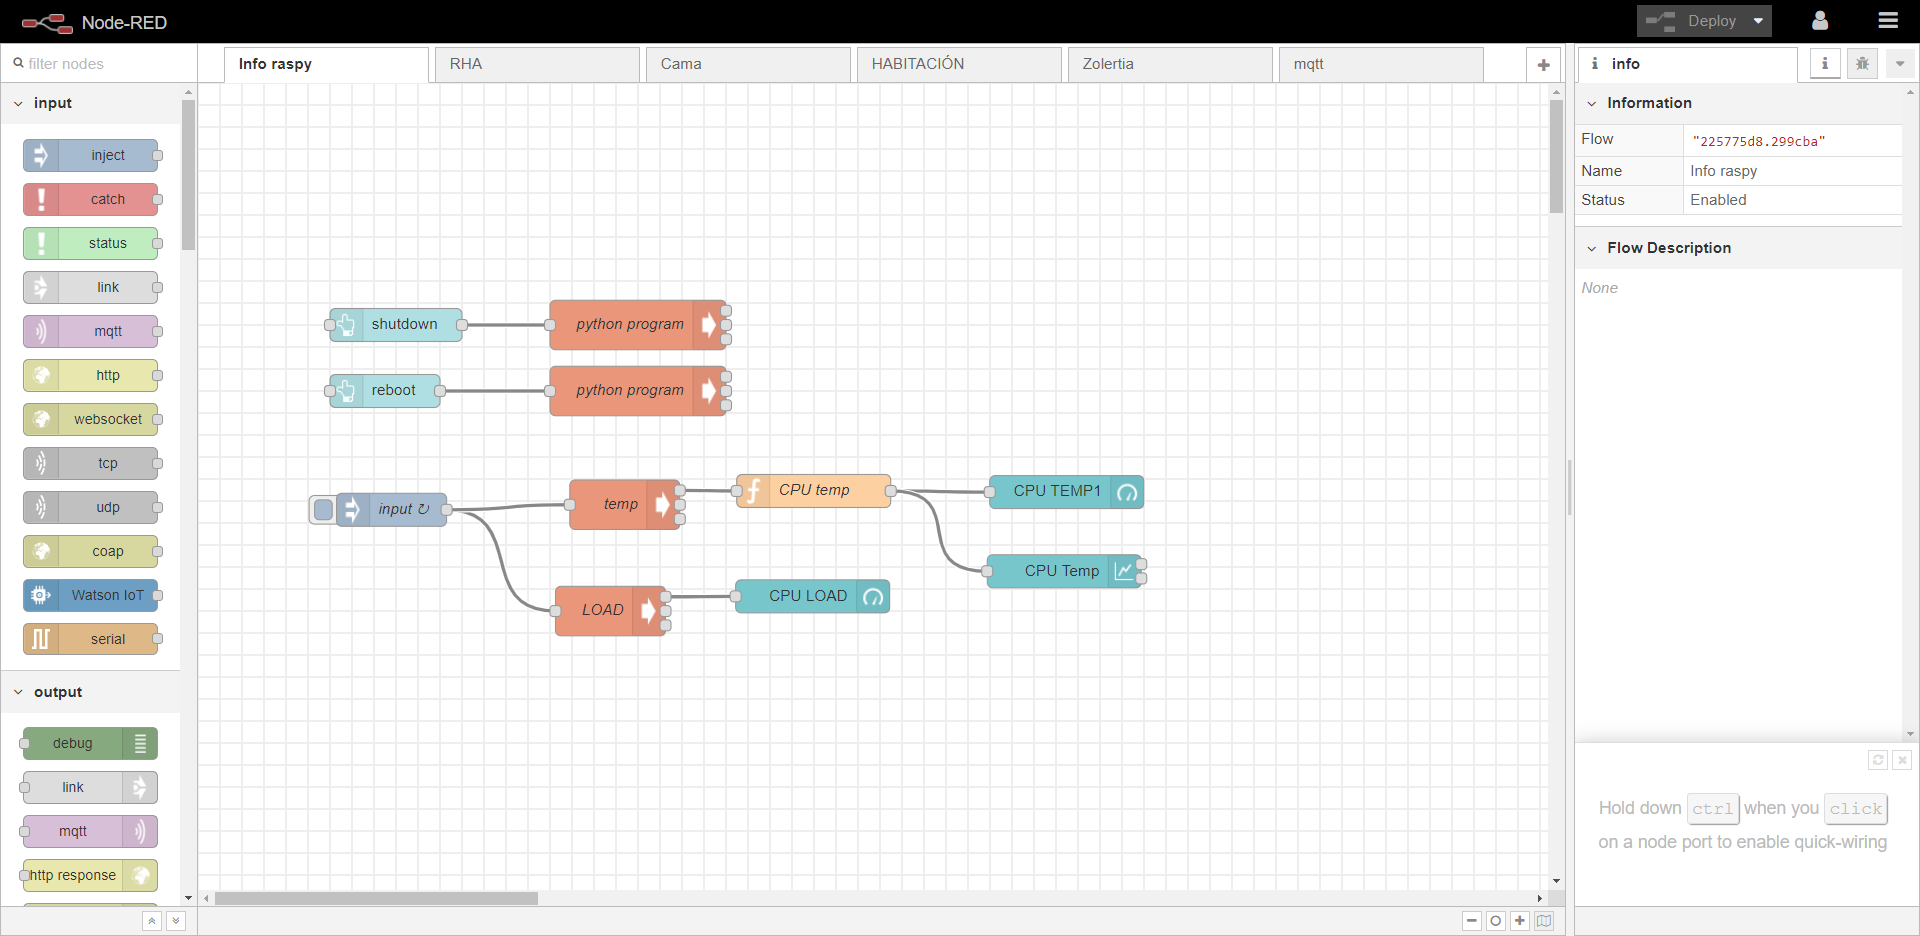
\includegraphics[width=0.7\textwidth]{figuras/InterfazNodeRed.png}
\caption{Ejemplo de interfaz de Node-RED}
\label{fig:nodeinterfaz}
\end{figure}

\begin{itemize}
\item \textbf{Debug node}

El nodo \textit{Debug} (figura \ref{fig:nodedebug}) representa una imagen del objeto \textit{msg} o de uno de sus atributos a su paso por un punto concreto del flujo. Normalmente hace uso de la pestaña debug de la interfaz de Node-RED.

\begin{figure}[H]
  \centering
  \begin{minipage}[b]{0.3\textwidth}
    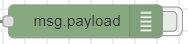
\includegraphics[width=\textwidth]{figuras/debugNode.png}
    \subcaption{Representación}
  \end{minipage}
  \hfill
  \begin{minipage}[b]{0.5\textwidth}
    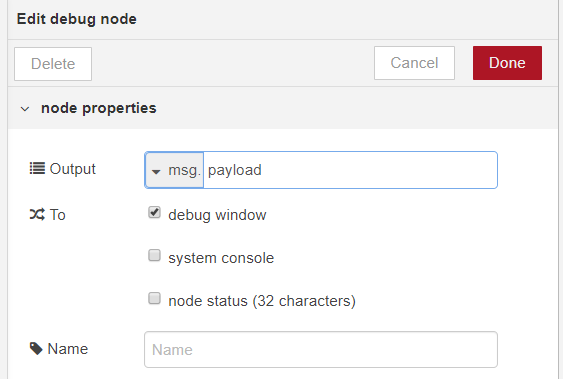
\includegraphics[width=\textwidth]{figuras/debugNodeProp.png}
    \subcaption{Configuración}
  \end{minipage}
  \caption{Nodo Debug}\label{fig:nodedebug}
\end{figure}

\item \textbf{Function node}

El nodo \textit{Function} (figura \ref{fig:nodefunction}) contiene una función programada en JavaScript que, por convenio, recibe el objeto \textit{msg} proveniente del flujo y lo utiliza para crear un nuevo objeto (u objetos) \textit{message} que pasar al siguiente nodo del flujo. Existe la posibilidad de no devolver nada si se desea congelar el flujo en ciertas situaciones.

\begin{figure}[H]
\centering
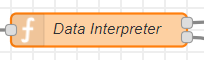
\includegraphics[width=0.5\textwidth]{figuras/fcnNode.png}
\caption{Nodo Function}
\label{fig:nodefunction}
\end{figure}

\item \textbf{Exec node}

El nodo \textit{Exec} (figura \ref{fig:nodeexec}) es el nodo de ejecución de comandos. El comando a ejecutar se define en las propiedades, siendo posible añadir el mensaje recibido a través del flujo al final del comando. Las salidas del bloque corresponden a \textit{stdout}, \textit{stderr} y a objetos devueltos. Es posible configurar si la salida debe volcarse al final de la ejecución o en directo durante la ejecución del programa.

\begin{figure}[H]
  \centering
  \begin{minipage}[b]{0.3\textwidth}
    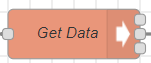
\includegraphics[width=\textwidth]{figuras/execNode.png}
    \subcaption{Representación}
  \end{minipage}
  \hfill
  \begin{minipage}[b]{0.5\textwidth}
    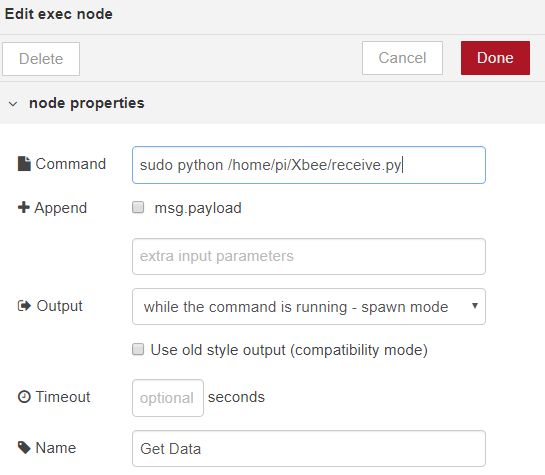
\includegraphics[width=\textwidth]{figuras/execNodeProp.png}
    \subcaption{Configuración}
  \end{minipage}
  \caption{Nodo Debug}\label{fig:nodeexec}
\end{figure}

\item \textbf{MQTT node}

Algunos de los nodos desarrollados por terceros son los relacionados con MQTT. Existen nodos de entrada de MQTT (figura \ref{fig:nodeMQTT}) y nodos de salida. La configuración disponible incluye la IP, el puerto y el \textit{topic} al que suscribirse o publicar.

\begin{figure}[H]
  \centering
  \begin{minipage}[b]{0.3\textwidth}
    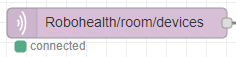
\includegraphics[width=\textwidth]{figuras/MQTTNode.png}
    \subcaption{Representación}
  \end{minipage}
  \hfill
  \begin{minipage}[b]{0.5\textwidth}
    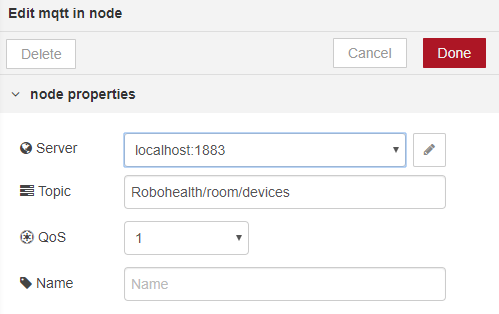
\includegraphics[width=\textwidth]{figuras/MQTTNodeProp.png}
    \subcaption{Configuración}
  \end{minipage}
  \caption{Nodo entrada MQTT}\label{fig:nodeMQTT}
\end{figure}

\item \textbf{Nodos de gestión de flujo}

Una serie de nodos se usan para modificar el comportamiento normal del flujo de los mensajes \textit{msg}. Posibilitan la aplicación de cierta lógica al programa.

\begin{itemize}

\item \textbf{Inject node}

El nodo de inyección introduce un mensaje en el flujo. Se puede programar una inyección periódica, que haga funcionar el flujo de manera similar a un bucle software.

\begin{figure}[H]
  \centering
  \begin{minipage}[b]{0.3\textwidth}
    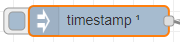
\includegraphics[width=\textwidth]{figuras/injectNode.png}
    \subcaption{Representación}
  \end{minipage}
  \hfill
  \begin{minipage}[b]{0.5\textwidth}
    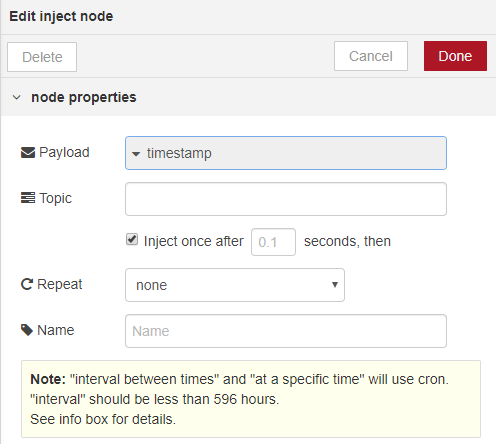
\includegraphics[width=\textwidth]{figuras/injectNodeProp.png}
    \subcaption{Configuración}
  \end{minipage}
  \caption{Nodo Inject}\label{fig:nodeinject}
\end{figure}

\item \textbf{Delay node}

El nodo \textit{Delay} detiene la ejecución del programa durante el tiempo especificado.

\begin{figure}[H]
  \centering
  \begin{minipage}[b]{0.3\textwidth}
    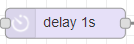
\includegraphics[width=\textwidth]{figuras/delayNode.png}
    \subcaption{Representación}
  \end{minipage}
  \hfill
  \begin{minipage}[b]{0.5\textwidth}
    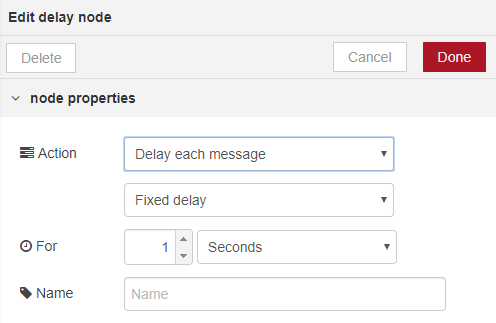
\includegraphics[width=\textwidth]{figuras/delayNodeProp.png}
    \subcaption{Configuración}
  \end{minipage}
  \caption{Nodo Delay}\label{fig:nodedelay}
\end{figure}

\item \textbf{Switch node}

El nodo \textit{Switch} compara algún atributo del mensaje \textit{msg} con unos valores programados y asignados a cada una de las salidas. Es equivalente a la expresión condicional \textit{switch-case}.

\begin{figure}[H]
  \centering
  \begin{minipage}[b]{0.3\textwidth}
    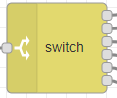
\includegraphics[width=\textwidth]{figuras/switchNode.png}
    \subcaption{Representación}
  \end{minipage}
  \hfill
  \begin{minipage}[b]{0.5\textwidth}
    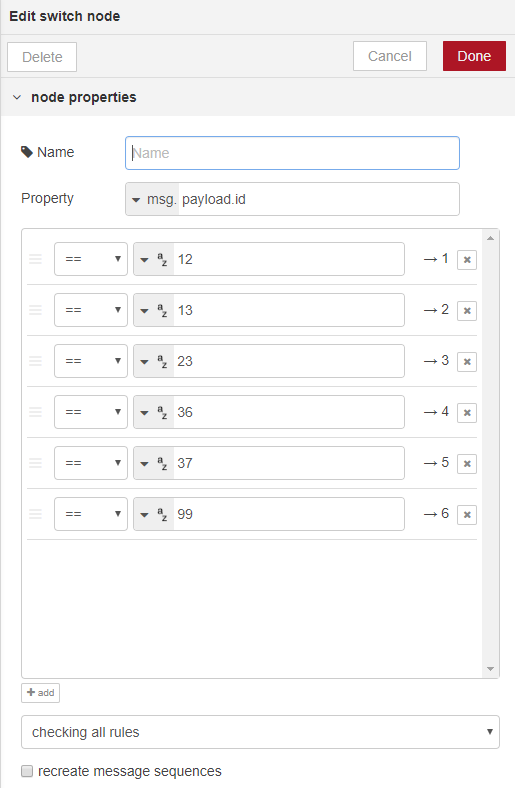
\includegraphics[width=\textwidth]{figuras/switchNodeProp.png}
    \subcaption{Configuración}
  \end{minipage}
  \caption{Nodo Switch}\label{fig:nodeexec}
\end{figure}

\end{itemize}


\item \textbf{Nodos de UI}

Existen varios nodos que representan objetos en el Dashboard de Node-RED que sirve de interfaz gráfica. Estos nodos pueden ser de entrada o salida de información

\begin{itemize}
\item \textbf{Ejemplos de nodos de entrada}

Los nodos de entrada (figura \ref{fig:nodeinput}) permiten introducir mensajes en el sistema. Existen entradas digitales, como pueden ser botones o interruptores, o entradas analógicas, como sliders.

\begin{figure}[H]
  \centering
  \begin{minipage}[t]{0.3\textwidth}
    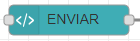
\includegraphics[width=\textwidth]{figuras/templateNode.png}
    \subcaption{Nodo Template}
  \end{minipage}
  \hfill
  \begin{minipage}[t]{0.4\textwidth}
    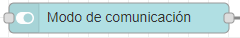
\includegraphics[width=\textwidth]{figuras/switchinputNode.png}
    \subcaption{Nodo interruptor}
  \end{minipage}
  \begin{minipage}[b]{0.3\textwidth}
    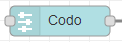
\includegraphics[width=\textwidth]{figuras/sliderNode.png}
    \subcaption{Nodo Slider}
  \end{minipage}
  \hfill
  \begin{minipage}[b]{0.3\textwidth}
    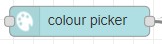
\includegraphics[width=\textwidth]{figuras/colourNode.png}
    \subcaption{Nodo selector de color}
  \end{minipage}
  \caption{Nodos de entrada}\label{fig:nodeinput}
\end{figure}

\item \textbf{Ejemplos de nodos de salida}

Los nodos de salida (figura \ref{fig:nodeoutput}) representan el valor de algún atributo del mensaje que les llega. Esta representación puede tener formato de texto, numérico o gráfico.

\begin{figure}[H]
  \centering
  \begin{minipage}[t]{0.3\textwidth}
    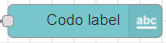
\includegraphics[width=\textwidth]{figuras/textNode.png}
    \subcaption{Nodo de texto}
  \end{minipage}
  \hfill
  \begin{minipage}[t]{0.3\textwidth}
    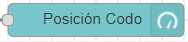
\includegraphics[width=\textwidth]{figuras/gaugeNode.png}
    \subcaption{Nodo gráfico}
  \end{minipage}
  \hfill
  \begin{minipage}[t]{0.3\textwidth}
    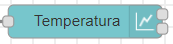
\includegraphics[width=\textwidth]{figuras/chartNode.png}
    \subcaption{Nodo Chart}
  \end{minipage}
  %\hfill
  \caption{Nodos de salida}\label{fig:nodeoutput}
\end{figure}

\end{itemize}
\end{itemize}

\subsubsection{Node-RED en RoboHealth}

La aplicación de Node-RED para los dispositivos de RoboHealth se orienta a la interacción con el usuario a través de una interfaz gráfica. Esta interfaz gráfica se divide en dos layout.

El primer layout (figura \ref{fig:infoRaspyDash}) se encarga del control básico del estado de la Raspberry Pi. Incluye representaciones de la temperatura y el uso de la CPU así como botones para reiniciar y apagar el ordenador.

\begin{figure}[H]
\centering
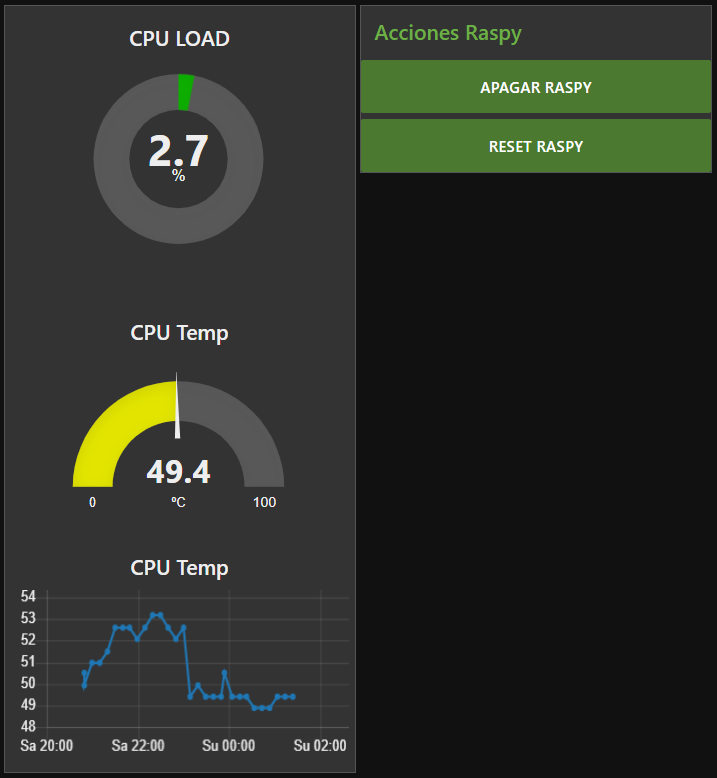
\includegraphics[width=0.7\textwidth]{figuras/infoRaspyDash.png}
\caption{UI de control elemental}
\label{fig:infoRaspyDash}
\end{figure}

El flujo (figura \ref{fig:infoRaspyFlow}) se basa en la ejecución de comandos para obtener la información de temperatura (línea 1/código \ref{comando:infoRaspy}) y carga de la CPU (línea 2/código \ref{comando:infoRaspy}). De igual manera, se lanzan comandos para apagar (línea 3/código \ref{comando:infoRaspy}) y reiniciar (línea 4/código \ref{comando:infoRaspy}) la Raspberry Pi. Los comandos utilizados son los siguientes:

% Configuración de la visualización del código SW
\lstset{backgroundcolor=\color{verde_p},numbers=left,numberstyle=\tiny, language=bash, breaklines=true, basicstyle=\footnotesize, xleftmargin=25pt, framesep=8pt, numbersep=15pt}

\begin{lstlisting}[frame=single, label=command:ssh, label=comando:infoRaspy]
$ vcgencmd measure_temp
$ top -d 0.5 -b -n2 | grep "Cpu(s)"|tail -n 1 | awk '{print $2 + $4}'
$ sudo shutdown -h now
$ sudo reboot
\end{lstlisting}

\begin{figure}[tb]
\centering
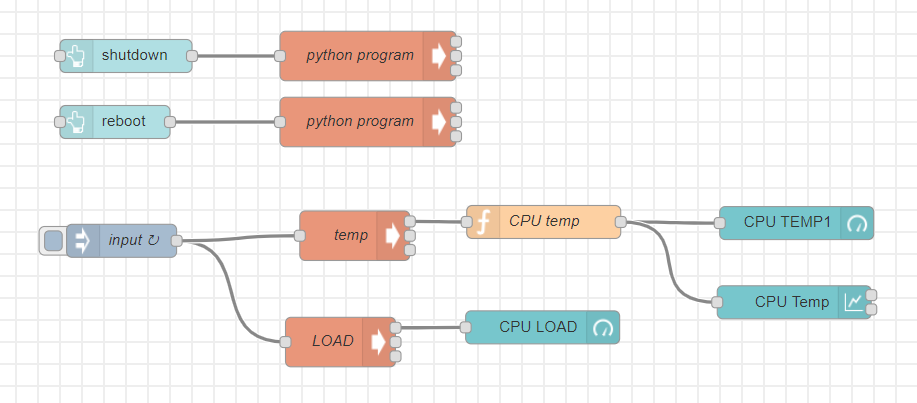
\includegraphics[width=0.9\textwidth]{figuras/infoRaspyFlow.png}
\caption{Flujo de control elemental}
\label{fig:infoRaspyFlow}
\end{figure}

El segundo layout incluye el control de los dispositivos previamente desarrollado. El Dashboard (figura \ref{fig:Dashboard}) recoge la UI para controlar cada bloque de dispositivos. A continuación se recogen ejemplos de los flujos correspondientes a la cama (figura \ref{fig:camaFlow}), la habitación (figura \ref{fig:persianasFlow}\footnote{En la imagen se recoge únicamente el flujo correspondiente a las persianas}) o los dispositivos Zolertia (figura \ref{fig:zolertiaFlow}).

\begin{figure}[tb]
\centering
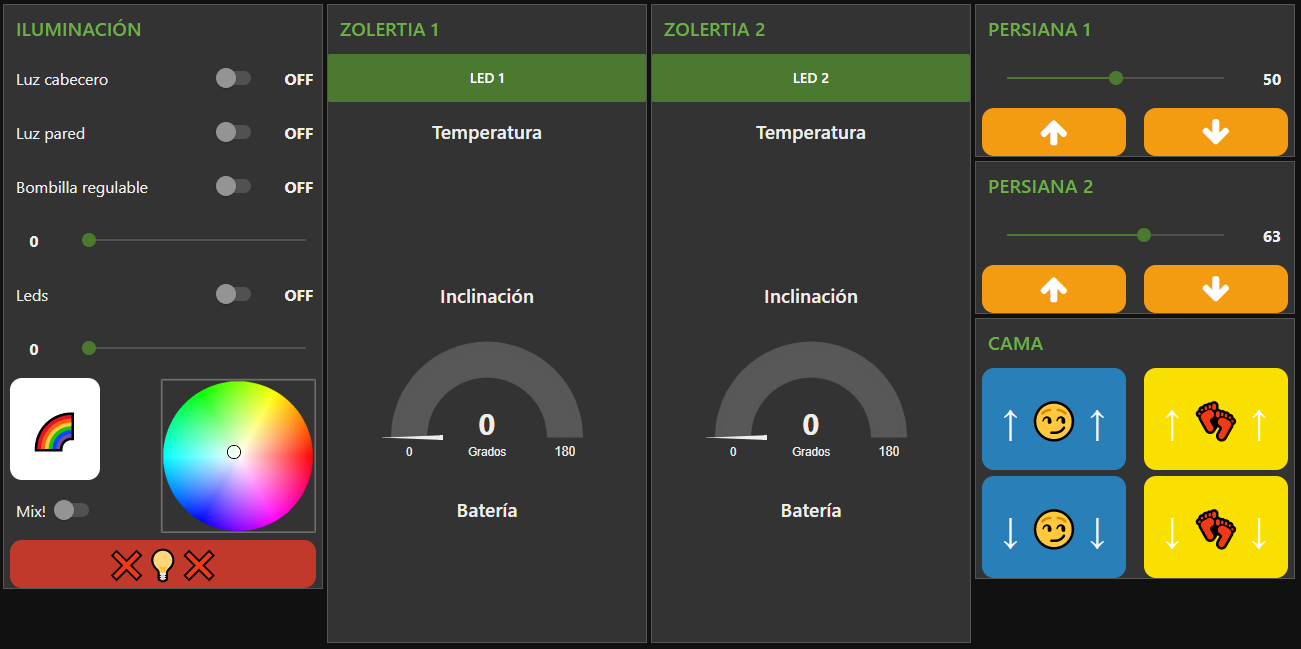
\includegraphics[width=0.8\textwidth]{figuras/Dashboard.png}
\caption{Dashboard}
\label{fig:Dashboard}
\end{figure}

\begin{figure}[H]
\centering
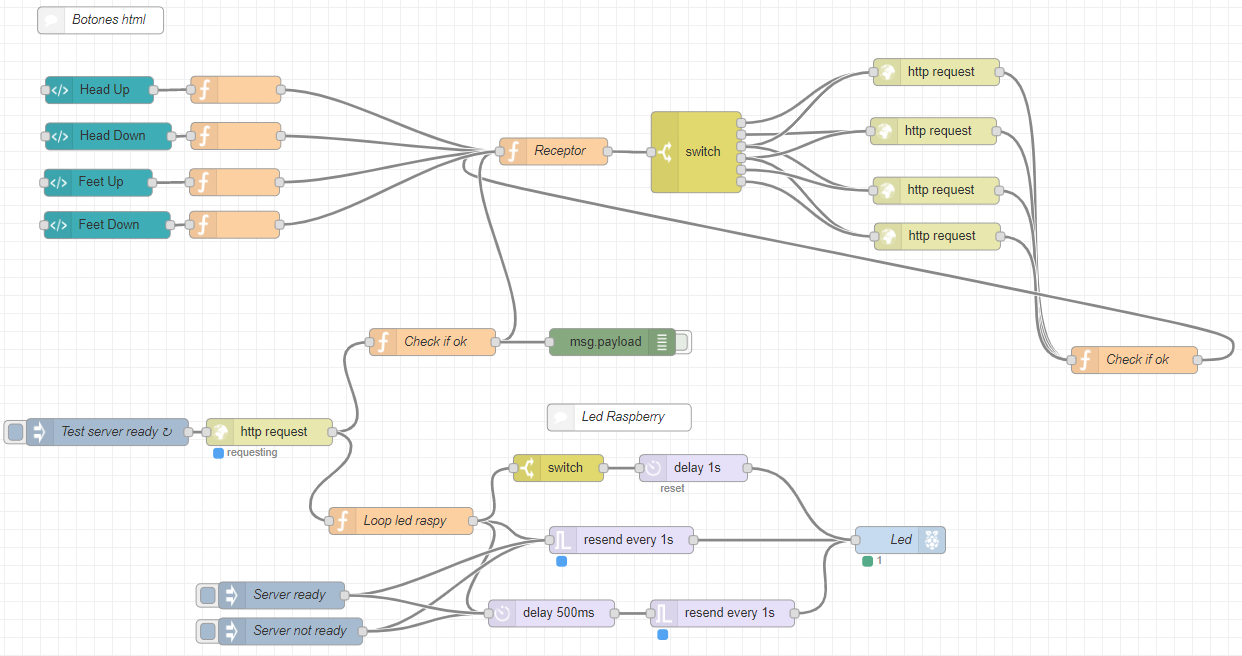
\includegraphics[width=1\textwidth]{figuras/camaFlow.png}
\caption{Flujo de control de la cama}
\label{fig:camaFlow}
\end{figure}

\begin{figure}[H]
\centering
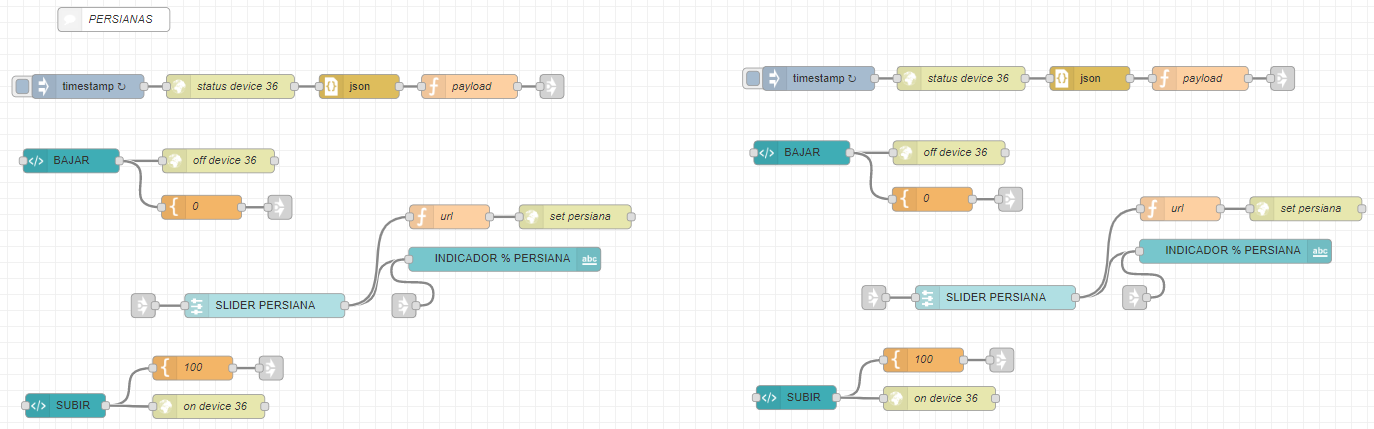
\includegraphics[width=1\textwidth]{figuras/persianasFlow.png}
\caption{Flujo de control de las persianas}
\label{fig:persianasFlow}
\end{figure}

\begin{figure}[H]
\centering
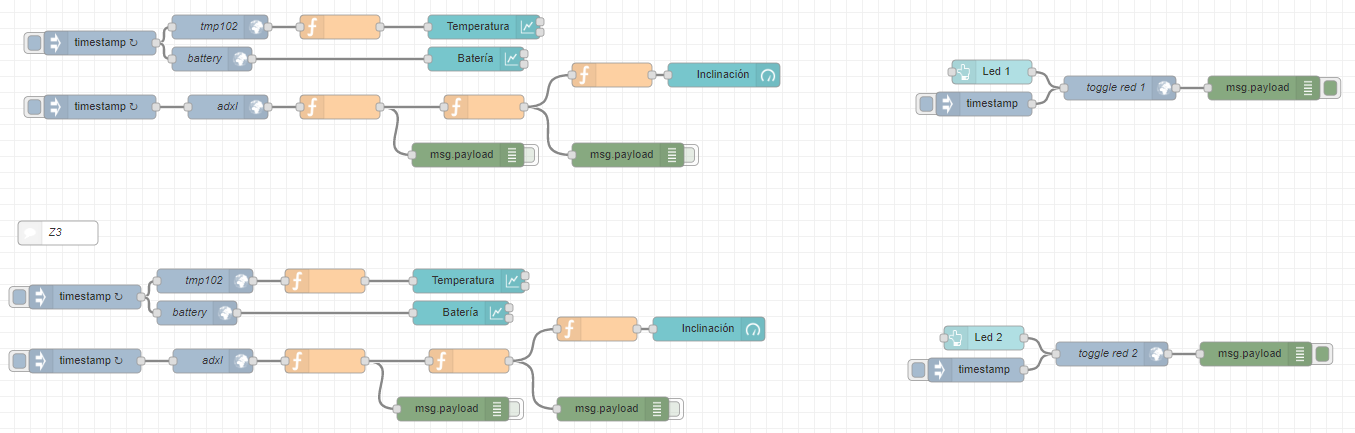
\includegraphics[width=1\textwidth]{figuras/zolertiaFlow.png}
\caption{Flujo de control de Zolertia}
\label{fig:zolertiaFlow}
\end{figure}

\subsubsection{Node-RED para RoboHealth Arm}

Para el control de RoboHealth Arm se ha desarrollado un flujo en Node-RED que se explica a continuación.

En la figura \ref{fig:ONOFFRHA} se muestra el flujo de encendido del brazo robótico

\begin{figure}[H]
\centering
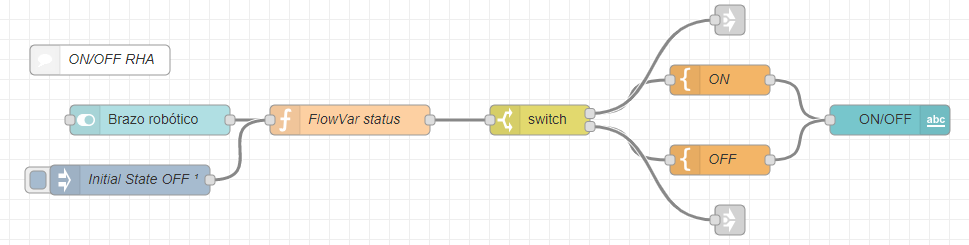
\includegraphics[width=0.9\textwidth]{figuras/ONOFFFlowRHA.png}
\caption{Flujo de encendido de RHA}
\label{fig:ONOFFRHA}
\end{figure}

El flujo se basa en la obtención el estado del control del brazo a través del botón ON/OFF y su asignación a una variable de flujo. Esta asignación se efectúa a través de la función \textit{FlowVar status} (código \ref{code:FlowVarStatus})

% Esto para configurar como se va a visualizar el código
\lstset{backgroundcolor=\color{amarillo_claro}, numbers=left,numberstyle=\tiny, language=Java, breaklines=true, basicstyle=\footnotesize, xleftmargin=25pt, framesep=8pt, numbersep=15pt}


\begin{lstlisting}[frame=leftline, caption={FlowVar status}, label=code:FlowVarStatus]
if (msg.payload === true) {
    flow.set("status","ON");
}
else if (msg.payload === false) {
    flow.set("status","OFF");
}
msg.payload = flow.get("status");
return msg;
\end{lstlisting}

Se incluye también en el flujo la inyección del estado inicial OFF al comenzar la ejecución.

El flujo de recepción de la información de RHA se programa como en la figura \ref{fig:RecepcionRHA}

\begin{figure}[H]
\centering
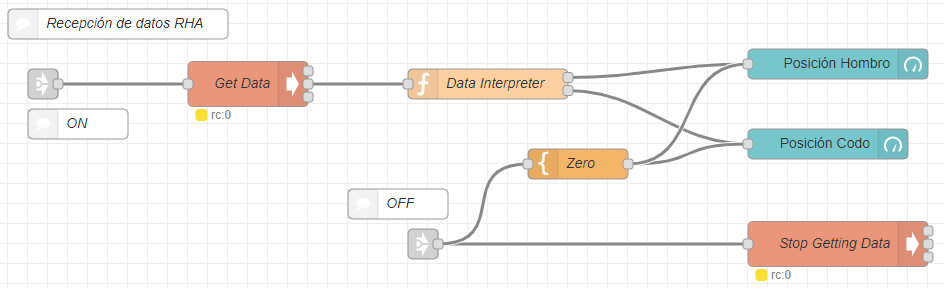
\includegraphics[width=0.9\textwidth]{figuras/RecepcionFlowRHA.png}
\caption{Flujo de recepción de RHA}
\label{fig:RecepcionRHA}
\end{figure}

La recepción de un flanco de encendido, pone a correr el comando \ref{command:getDataRHA} que lanza un script que devuelve los datos recibidos. Estos datos se interpretan con la función \textit{Data interpreter} (código \ref{code:DataInterpreter}) y se muestra la información en el Dashboard con una salida gráfica

% Configuración de la visualización del código SW
\lstset{backgroundcolor=\color{verde_p}, numbers=none, language=bash, breaklines=true, basicstyle=\footnotesize, xleftmargin=25pt, framesep=8pt, numbersep=15pt}

\begin{lstlisting}[frame=single, label=command:getDataRHA]
$ sudo python /home/pi/Xbee/receive.py
\end{lstlisting}

% Esto para configurar como se va a visualizar el código
\lstset{backgroundcolor=\color{amarillo_claro}, numbers=left,numberstyle=\tiny, language=Java, breaklines=true, basicstyle=\footnotesize, xleftmargin=25pt, framesep=8pt, numbersep=15pt}

\begin{lstlisting}[frame=leftline, caption={Data Interpreter}, label=code:DataInterpreter]
var num1_str = msg.payload[1]+msg.payload[2]+msg.payload[3];
if (msg.payload.length < 11) {
    var num2_str = msg.payload[6]+msg.payload[7];
}
else {
    var num2_str = msg.payload[6]+msg.payload[7]+msg.payload[8];
}
msg.payload = num1_str;
var newMsg = {payload: num2_str}
return [msg, newMsg];
\end{lstlisting}

Un flanco de apagado detiene el script con el comando \ref{comand:stopGettingDataRHA} y manda un 0 a la representación de la información

% Configuración de la visualización del código SW
\lstset{backgroundcolor=\color{verde_p}, numbers=none, language=bash, breaklines=true, basicstyle=\footnotesize, xleftmargin=25pt, framesep=8pt, numbersep=15pt}

\begin{lstlisting}[frame=single, label=command:stopGettingDataRHA]
$ sudo pkill -f receive.py
\end{lstlisting}

El flujo de configuración de la emisión de datos se encuentra en la figura \ref{fig:configRHA}. En resumen, obtiene los datos de posiciones articulares y modo de comunicación de la interfaz gráfica y los asigna a variables de flujo. Las posiciones articulares están limitadas por los slider: para el codo, los valores estan entre \textbf{60 y 110}; para el hombro, entre \textbf{125 y 166}. Las funciones \textit{FlowVar elbow}, \textit{FlowVar shoulder} y \textit{FlowVar ComMode} son similares a \textit{FlowVar status} (código \ref{code:FlowVarStatus}). El flujo también establece los valores iniciales para codo, hombro y modo de comunicación; siendo 60, 125 y AT respectivamente.

\begin{figure}[H]
\centering
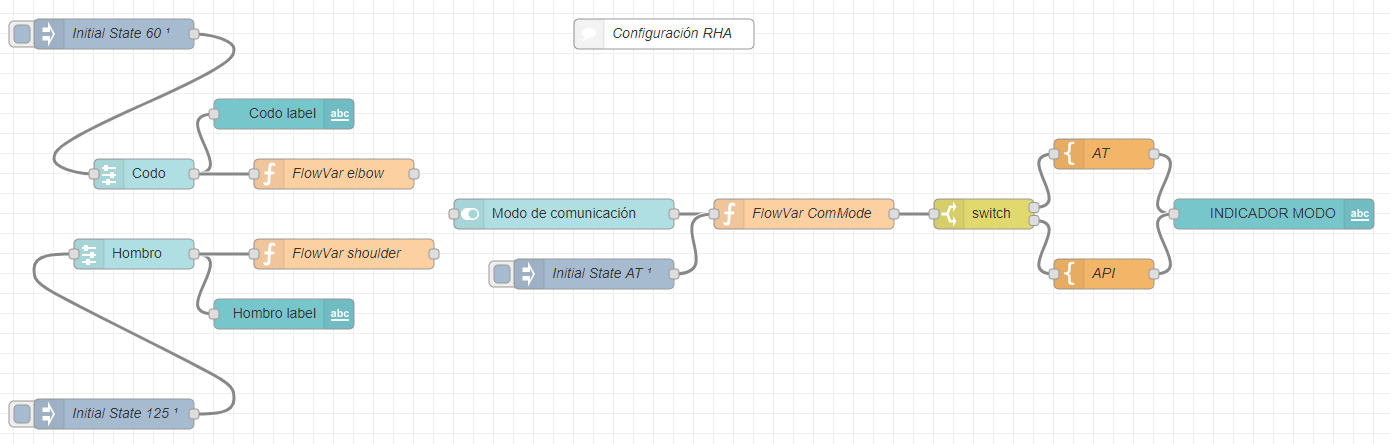
\includegraphics[width=0.9\textwidth]{figuras/configFlowRHA.png}
\caption{Flujo de configuración de RHA}
\label{fig:configRHA}
\end{figure}

En la figura \ref{fig:emisionRHA} se recoge el flujo correspondiente a la emisión de datos al RHA. Comprueba el tipo de comunicación y elige el script a correr de acuerdo a ello. Previamente, obtiene las coordenadas articulares para pasárselas a los scripts.

\begin{figure}[H]
\centering
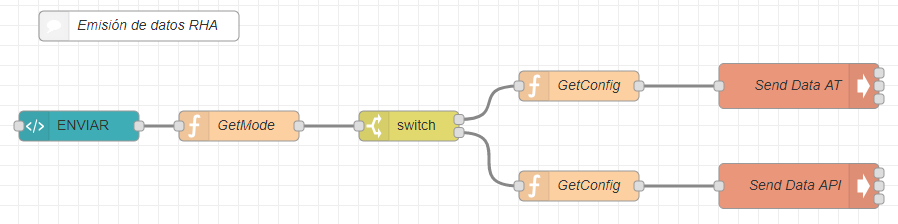
\includegraphics[width=0.9\textwidth]{figuras/emisionFlowRHA.png}
\caption{Flujo de emisión de RHA}
\label{fig:emisionRHA}
\end{figure}

Función \textit{GetMode}:

% Esto para configurar como se va a visualizar el código
\lstset{backgroundcolor=\color{amarillo_claro}, numbers=left,numberstyle=\tiny, language=Java, breaklines=true, basicstyle=\footnotesize, xleftmargin=25pt, framesep=8pt, numbersep=15pt}

\begin{lstlisting}[frame=leftline, caption={GetMode}, label=code:GetMode]
if (flow.get("ComMode") === undefined) {
    flow.set("ComMode","AT");
}
if (flow.get("status") == "ON") {
    msg.payload = flow.get("ComMode");
}
return msg;
\end{lstlisting}

Función \textit{GetConfig}:

\begin{lstlisting}[frame=leftline, caption={GetConfig}, label=code:GetConfig]
var posX = flow.get("RHA_shoulder");
var posY = flow.get("RHA_elbow");
var hex_posX = posX.toString(16);
var hex_posY = posY.toString(16);
msg.payload = [hex_posX,hex_posY];
return msg;
\end{lstlisting}

Los comandos para enviar los mensajes AT y API son los siguientes. En la práctica, \textit{msg.payload} se añade al final del comando, indicando la información a enviar.

% Configuración de la visualización del código SW
\lstset{backgroundcolor=\color{verde_p}, numbers=none, language=bash, breaklines=true, basicstyle=\footnotesize, xleftmargin=25pt, framesep=8pt, numbersep=15pt}

\begin{lstlisting}[frame=single, label=command:sendDataRHA]
$ sudo python /home/pi/Xbee/sendAT.py
$ sudo python /home/pi/Xbee/sendAPI.py
\end{lstlisting}

El resultado gráfico de todos estos nodos y flujos se plasma en una interfaz de usuario como la de la figura \ref{fig:DashRHA}.

\begin{figure}[H]
\centering
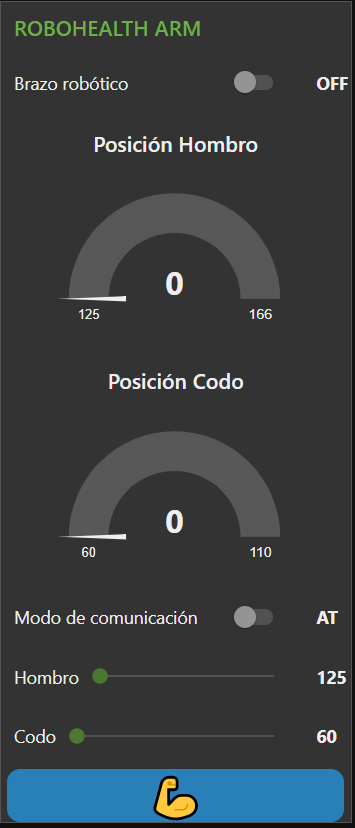
\includegraphics[width=0.5\textwidth]{figuras/DashRHA.png}
\caption{Dashboard para el control de RHA}
\label{fig:DashRHA}
\end{figure}

Se puede observar un switch de ON/OFF para habilitar o deshabilitar la emisión y recepción de información. Las coordenadas articulares de hombro y codo son representadas mientras se actualizan en directo. Hay otro switch para seleccionar el moto de transmisión de datos y, por último, dos sliders para seleccionar una posición objetivo y un botón para lanzar la información al brazo robótico.


\section{Transmisión de la información}

Para la transmisión de la información, se eligió utilizar tecnología basada en la radiofrecuencia con el objetivo de diversificar la naturaleza de los dispositivos presentes en la habitación del proyecto RoboHealth.

Dentro de la radiofrecuencia, existen varios tipos de dispositivos y plataformas que pueden ayudarnos en nuestro objetivo. Un resumen de estas alternativas con sus características puede ser encontrado en la tabla \ref{tab:radio}.

\begin{table}[H]
\begin{center}
\begin{tabular}{|m{3cm}|m{1cm}|m{7cm}|}
\hline
\textbf{Nombre} & \multicolumn{2}{|c|}{\textbf{Características}}\\
\hline
\hline
\multirow{2}{3cm}{XBee} & Pros & Mucha documentación, variedad de versiones, precio contenido, versatilidad\\
\cline{2-3}
& Cons & Sobredimensionado\\
\hline
\multirow{2}{3cm}{Jennic JN5148} & Pros & Menor tamaño, coste contenidos\\
\cline{2-3}
& Cons & Dificil distribución, documentación limitada\\
\hline
\multirow{2}{3cm}{HPZB01W} & Pros & Precio contenido\\
\cline{2-3}
& Cons & Comunicación lenta, difícil manejo y escasa documentación\\
\hline
\multirow{2}{3cm}{RFM12B} & Pros & Coste muy reducido\\
\cline{2-3}
& Cons & Escasa potencia, muy pequeña versatilidad\\
\hline
\end{tabular}
\end{center}
\caption{Alternativas de radiofrecuencia}
\label{tab:radio}
\end{table}

Finalmente, se decidió optar por los módulos XBee. Además de que sus características los hacen perfectamente funcionales para el desarrollo del presente proyecto y las alternativas no eran especialmente buenas, el departamento ya contaba con un par de estos módulos.

\subsection{Módulos XBee}

Los módulos XBee \cite{Xbee:2019} (figura \ref{fig:Xbee}) son un conjunto de pequeños productos orientados a solucionar redes inalámbricas para la comunicación entre dispositivos. Entre sus características se encuentran:

\begin{itemize}
\item Gran variedad de productos que recorren un rango muy amplio tanto de consumos de potencia como de alcances.
\item Son módulos que ofrecen un alto tráfico de datos
\item Baja latencia en la comunicación
\item Precisan una sicronización de comunicación predecible
\item Su aplicación principal es la creación de redes \textit{punto a punto} o \textit{punto a multipunto}.
\end{itemize}

Los módulos XBee trabajan sobre la especificación \textbf{Zigbee} \cite{Zigbee:2019}, que proporciona una alianza y un estandar sobre el que trabajar en redes \textit{mesh} de comunicación. Esta especificación se basa en el estándar IEEE 802.15.4 \cite{IEEE:2007}, que define características físicas como el mecanismo DSSS para la modulación en radiofrecuencia (Se pueden encontrar más detalles en la sección \ref{sec:radiofrec}).

Los módulos XBee de los que se disponen son los denominados XBee S2\cite{XbeeS2:2007}, permiten dos modos de comunicación (apartado \ref{subsubsec:modoscom}) y una infinidad de parámetros configurables (apartado \ref{subsubsec:xctu}). Estos módulos sólo funcionan con módulos de la mismo Serie 2, por lo que todos los dispositivos miembros de la red deben incluir este tipo de módulos.

El módulo XBee S2 trabaja a 3.3V de tensión de alimentación, el layout físico puede consultarse en la figura \ref{fig:XBLayout} y su pinout puede encontrarse en la figura \ref{fig:XBPinout}.

\begin{figure}[tb]
\centering
\includegraphics[width=0.5\textwidth]{figuras/XBeeLayout.png}
\caption{Layout del XBee S2}
\label{fig:XBLayout}
\end{figure}

\begin{figure}[bt]
\centering
\includegraphics[width=0.9\textwidth]{figuras/XBeePinout.png}
\caption{Pinout del XBee S2}
\label{fig:XBPinout}
\end{figure}

Toda la información relacionada con los módulos de radiofracuencia de Digi puede consultarse en el PDF destinado a ello\cite{Digi:2018} que puede encontrarse en internet.

\subsubsection{Modos de comunicación}\label{subsubsec:modoscom}

Como se ha comentado con anterioridad, existen dos modos de comunicación que pasan a desarrollarse a continuación. Es destacable el hecho de que los modos de comunicación deben coincidir entre los extremos comunicados para que la interpretación o el propio proceso de comunicación sea efectivo.

\begin{itemize}
\item \textbf{Modo AT}

En el modo AT o modo transparente, el módulo actúa como una simple sustitución de la comunicación serial.

Cuando cualquier tipo de información es recibida por radiofrecuencia, es directamente trasladada al pin DOUT del módulo.

Cuando se recibe información a través del pin DIN, se transmite por radiofrecuencia drectamente a las direcciones definidas en la configuración (apartado \ref{subsubsec:xctu}).

Este método es el más simple pero, si en la red existen más de dos módulos XBee y se quiere discriminar la transmisión de información entre uno y otro, los módulos requieren ser reconfigurados a través de los registros de las direcciones de destino. En ese caso, limita mucho la facilidad de la operación.

Se puede comprobar que el script SendAT.py (apartado \ref{subsubsec:sendat}) envía exclusivamente los bytes correspondientes al protocolo de comunicación RHA. La recepción (apartado \ref{subsubsec:receive}) también está pensado para recibir en modo AT, ya que se trata de ser lo menos intrusivo posible en el código fuente del brazo robótico y éste no está preparado para transmitir en modo API.

\item \textbf{Modo API}

El modo API (\textit{Application Programming Interface}) es una alternativa al modo transparente que enmarca la emisión de datos en una serie de mensajes estandarizados. La tabla \ref{tab:APIFrame} recoge la estructura de un API Frame. Todos los mensajes usados a través de este modo deberán atenerse a esta estructura.

\begin{table}[bt]
\begin{center}
\begin{tabular}{|m{20mm}|m{10mm}|m{10mm}|m{10mm}|m{5mm}|m{5mm}|m{5mm}|m{5mm}|m{5mm}|m{5mm}|m{5mm}|m{20mm}|}
\hline
\textbf{Encabezado} & \multicolumn{2}{|c|}{\textbf{Longitud}} & \textbf{Tipo} & \multicolumn{7}{|c|}{\textbf{Datos}} & \textbf{Checksum}\\
\hline
\hline
1 & 2 & 3 & 4 & 5 & 6 & 7 & 8 & 9 & ... & n & n+1\\
\hline
0x7E & MSB & LSB & Tipo & \multicolumn{7}{|c|}{Información específica del tipo de Frame} & Byte de Checksum\\
\hline
\end{tabular}
\end{center}
\caption{Estructura de un API Frame}
\label{tab:APIFrame}
\end{table}

En la figura \ref{fig:txAPI} se pueden ver los tipos de frames estandarizados para la transmisión de datos. De igual manera, los tipos de frames de recepción están recogidos en la figura \ref{fig:rxAPI}.

\begin{figure}[b]
\centering
\includegraphics[width=0.9\textwidth]{figuras/txAPIFrames.png}
\caption{API Frames de transmisión}
\label{fig:txAPI}
\end{figure}

\begin{figure}[H]
\centering
\includegraphics[width=0.9\textwidth]{figuras/rxAPIFrames.png}
\caption{API Frames de recepción}
\label{fig:rxAPI}
\end{figure}

Para que un módulo configurado en este modo pueda emitir datos por radio, la información recibida por DIN debe adecuarse a los frames preestablecidos.

Si bien este modo aumenta la complejidad de los frames transmitidos, tiene la ventaja de contener la dirección de destino en el propio frame. Esto permite filtrar los receptores del mensaje en el propio mensaje, sin necesidad de acceder a la configuración del módulo XBee. Además, es posible recibir feedback de la transmisión del mensaje ya que la recepción de unos tipos de mensaje provocan la emisión de vuelta de otros que indican su recepción.

En el script sendAPI.py (apartado \ref{subsubsec:sendapi}) se genera un API frame de tipo 0x10 \textit{Transmit Request}.

\end{itemize}

\subsubsection{Funciones de los módulos}

Existen tres posibles funciones de cada módulo XBee dependiendo de la posición que que ocupen en la red domótica. Cada función de XBee implica ligeros cambios en el firmware del módulo. En la figura \ref{fig:XbeeRed} se puede observar un ejemplo de red domótica usando XBee.



\begin{itemize}
\item \textbf{Coordinador}

El coordinador es el nodo central de la red. Su presencia en la red domótica es obligatoria y única (sólo se permite un nodo coordinador en la red). Se encarga de gestionar el resto de dispositivos, conecta y desconecta dispositivos de la red, asigna direcciones, traza mandatos y gestiona el consumo de energía pudiendo dormir al resto de dispositivos. Nunca puede apagarse o ponerse en modo de ahorro de energía.

\begin{figure}[H]
\centering
\includegraphics[width=0.9\textwidth]{figuras/XbeeRed.png}
\caption{Ejemplo de red XBee}
\label{fig:XbeeRed}
\end{figure}

En el caso del presente proyecto, se tratará del nodo unido a la Raspberry Pi, que funciona como unidad de mando.

\item \textbf{Router}

El Router es un nodo con funciones completas, puede mandar y recibir información. Puede unirse a redes existentes y se usa, principalmente, para extender la red domótica más alla del alcance del Coordinador. Se encarga de ser mensajero trasladando información desde el coordinador hasta \textit{End devices} u otros Routers; pudiendo llegar a modificar esta información.

Efectivamente, puede haber más de un router en la red y se encargan de gestionar los \textit{End devices} que tengan conectados, pudiéndoles poner en modo ahorro de energía. No pueden ponerse en modo ahorro de energía y deben estar encendidos todo el tiempo, como el coordinador

En el caso de la conexión de RHA, el XBee del brazo robótico tomará la función de router ya que precisa de una comunicación bidireccional con el Coordinador.

\item \textbf{End Device}

Los \textit{End Devices} son nodos extremos que pueden unirse a una red preexistente pero no pueden gestionar ningún dispositivo de ella. Pueden ponerse a ellos mismos en distintos modos de ahorro de energía. Las redes pueden tener un número muy alto de \textit{End Devices}, tantos como direcciones sean almacenables en el nodo coordinador.

Su uso suele estar orientado al envío de la medida de algún sensor.

\end{itemize}



\subsection{XBee Shield}

La XBee Shield (figura \ref{fig:XBeeSh}) es una solución que permite una interacción sencilla con los módulos XBee. Para ello, se basa en el uso de Arduino UNO (figura \ref{fig:AUno}. La XBee Shield posee un zócalo para situar el módulo XBee, está diseñada para encajar a la perfeccion sobre el Arduino UNO y esto descubre multitud de opciones.

Los diseños, layouts y planos son libres y pueden ser encontrados en internet. En el Anexo \ref{anexo:XBShield} se localiza el esquemático de la Xbee Shield.

Posee dos jumpers selectores que establecen el modo en el que debe comportarse la XBee Shield. El hecho de que haya dos es simplemente para asegurar un modo, ambos jumpers deben situarse en la misma posición para un correcto funcionamiento. La selección de estos modos configura la conexión entre la comunicación serial del módulo XBee y la comunicación serial entre el microcontrolador y el integrado USB-to-Serial de la Arduino UNO.

\subsubsection{Modo XBee}

Una de las posiciones de los jumpers es la posición XBee. En esta posición, el pin DOUT del módulo XBee se conecta al RX del microcontrolador y, por lo tanto, al TX del USB. Por otro lado, el pin DIN estaría conectado al TX del microcontrolador y, consecuentemente, al RX del USB.

Esta configuración permite que aquello que envíe el microcontrolador sea transmitido tanto por USB al ordenador como por radiofrecuencia. Sin embargo, la recepción de datos por parte del microcontrolador se realizará únicamente desde el módulo XBee, quedando inhabilitada el envío de datos por serial desde un ordenador.

Lógicamente, ya que se desea una comunicación bidireccional de datos con una Raspberry Pi, esta configuración queda descartada.

\subsubsection{Modo USB}\label{subsubsec:USBXB}

El otro modo alcanzable a través de los jumpers es el modo USB. Este modo consiste en la comunicación directa del pin DOUT del XBee al RX del USB y, por su parte, la conexión del pin DIN al TX del USB. 

Esto posibilita la conexión directa del módulo XBee al ordenador siempre que ningún otro dispositivo interfiera en la comunicación. Este dispositivo puede ser, perfectamente, el microcontrolador. Es esta la razón por la que es necesario retirar el microcontrolador del Arduino UNO para que funcione de manera adecuada el modo USB\footnote{De lo contrario, el Arduino UNO funcionaría de manera normal, ignorando el Modulo XBee}. Para retirar el microcontrolador, es necesario que la versión de Arduino UNO utilizada use el microcontrolador en su empaquetado de orificio pasante colocado sobre un zócalo. La versión SMD requiere desoldarlo y no termina de ser cómodo.

Puesto que en ninguno de los puntos del proyecto requerimos del preprocesamiento de los datos por un Arduino externo, el microcontrolador no aporta ninguna utilidad. Es la configuración USB, por lo tanto, la usada a lo largo del proyecto.

En concreto, hay una situacion en la que este modo adquiere especial sentido: a la hora de configurar el módulo y, en general, al usar XCTU con un módulo XBee. Se precisa una conexión directa Xbee-ordenador que la Xbee Shield en modo USB puede proporcionar.


\section{RoboHealth Arm}

RoboHealth Arm\cite{Heredia1:2018} (figura \ref{fig:RHA}) es un brazo robótico de tres grados de libertad cuyo sistema de acción se basa en un mecanismo controlado por una serie de cuerdas que son recogidas o liberadas por unos servos. Unos potenciónetros realimentan la posición de las dos articulaciones que funcionan con este mecanismo. El tercer grado de libertad, encargado de la rotación sobre su eje, no funciona de igual manera, sino que lo hace a través de un engranaje simple sin haber forma de realimentar su posición. Por lo tanto, el control de este tercer eje es absoluto.

\begin{figure}[bt]
\centering
\includegraphics[width=0.8\textwidth]{figuras/RHA.png}
\caption{RoboHealth Arm}
\label{fig:RHA}
\end{figure}

El programa que controla el brazo robótico\cite{Heredia2:2018} se carga sobre un microcontrolador Arduino Mega

RoboHealth Arm se trata de un Trabajo Final de Grado\cite{Heredia1:2018} realizado previamente en el marco del proyecto RoboHealth.

\subsection{Protocolo de comunicación RHA}

RoboHealth Arm incluye en su desarrollo un protocolo de comunicación detallado en \cite{Heredia1:2018}/Anexo E. Los mensajes enmarcados en este protocolo siguen la estructura recogida en la tabla \ref{tab:RHAcom}

\begin{table}[H]
\begin{center}
\begin{tabular}{|m{15mm}|m{15mm}|m{15mm}|m{15mm}|m{5mm}|m{5mm}|m{5mm}|m{5mm}|m{5mm}|m{20mm}|}
\hline
\multicolumn{2}{|c|}{\textbf{Encabezado}} & \textbf{Longitud} & \textbf{Tipo} & \multicolumn{5}{|c|}{\textbf{Parámetros}} & \textbf{Checksum}\\
\hline
\hline
1 & 2 & 3 & 4 & 5 & 6 & 7 & ... & n & n+1\\
\hline
0xFF & 0xFF & Longitud & Tipo & \multicolumn{5}{|c|}{Parámetros del mensaje} & Byte de Checksum\\
\hline
\end{tabular}
\end{center}
\caption{Estructura de un paquete genérico de comunicación RHA}
\label{tab:RHAcom}
\end{table}

En general, este proyecto se centra en dos tipos de mensajes.

\begin{itemize}
\item \textbf{Frame de estado}

Mensaje enviado de forma periódica desde el brazo informando de su estado. Como se puede apreciar en la estructura del frame recogida en la tabla \ref{tab:frameEstado}, permite conocer posición, velocidad y par de cada articulación.

\begin{table}[bth]
\begin{center}
\begin{tabular}{|m{15mm}|m{80mm}|}
\hline
\textbf{Byte} & \textbf{Información contenida}\\
\hline
0 & Encabezado (Fijo: 0xFF)\\
\hline
1 & Encabezado (Fijo: 0xFF)\\
\hline
2 & Longitud (0x06)\\
\hline
3 & Tipo (0x02)\\
\hline
4 & Objetivo de posición para la primera articulación\\
\hline
5 & Objetivo de posición para la segunda articulación\\
\hline
6 & Objetivo de posición para la tercera articulación\\
\hline
7 & \textit{Checksum}\\
\hline
\end{tabular}
\end{center}
\caption{Estructura del frame de comando\cite{Heredia1:2018}}
\label{tab:frameComando}
\end{table}

\begin{table}[bth]
\begin{center}
\begin{tabular}{|m{15mm}|m{60mm}|}
\hline
\textbf{Byte} & \textbf{Información contenida}\\
\hline
0 & Encabezado (Fijo: 0xFF)\\
\hline
1 & Encabezado (Fijo: 0xFF)\\
\hline
2 & Longitud a leer (18)\\
\hline
3 & Tipo de mensaje (0)\\
\hline
\multicolumn{2}{|c|}{\textbf{Información de la primera articulación}}\\
\hline
4 & Posición articular\\
\hline
5 & Velocidad (con dirección). Byte L\\
\hline
6 & Velocidad (con dirección). Byte H\\
\hline
7 & Par aplicado (con dirección). Byte L\\
\hline
8 & Par aplicado (con dirección). Byte H\\
\hline
\multicolumn{2}{|c|}{\textbf{Información de la segunda articulación}}\\
\hline
9 & Posición articular\\
\hline
10 & Velocidad (con dirección). Byte L\\
\hline
11 & Velocidad (con dirección). Byte H\\
\hline
12 & Par aplicado (con dirección). Byte L\\
\hline
13 & Par aplicado (con dirección). Byte H\\
\hline
\multicolumn{2}{|c|}{\textbf{Información de la tercera articulación}}\\
\hline
14 & Posición articular\\
\hline
15 & Velocidad (con dirección). Byte L\\
\hline
16 & Velocidad (con dirección). Byte H\\
\hline
17 & Par aplicado (con dirección). Byte L\\
\hline
18 & Par aplicado (con dirección). Byte H\\
\hline
19 & \textit{Checksum}\\
\hline
\end{tabular}
\end{center}
\caption{Estructura del frame de estado\cite{Heredia1:2018}}
\label{tab:frameEstado}
\end{table}

\item \textbf{Frame de comando}

Es el mensaje utilizado para comandar el brazo robótico. RHA está permanentemente leyendo la entrada serial. La codificación de este tipo de mensaje se muestra en la tabla \ref{tab:frameComando}.



\end{itemize}



\definecolor{verde_p}{rgb}{0.77,0.97,0.84}
\definecolor{amarillo_claro}{rgb}{1,1,0.90}

\chapter{Implementación del proyecto}

\section{Scripts en la Raspberry Pi}

En la Raspberry Pi están guardados una serie se scripts en lenguaje Python que son los encargados de enviar (tanto en modo AT, como en modo API) y recibir la información.

Unos comentarios sobre la edición y compilación de scripts escritos en Python en una máquina que corra Raspbian y, en general, cualquier sistema operativo basado en GNU/Linux, pueden ser encontrados en el Anexo \ref{anexo:scripts}.

A continuación se explica detalladamente cada uno de estos scripts.

\subsection{SendAT.py}\label{subsubsec:sendat}

Es un script encargado de enviar comandos en modo AT hacia el puerto serial adecuado. El \textbf{código íntegro de SendAT.py} se puede encontrar en el Anexo \ref{anexo:sendAT}.

En las primeras 5 líneas se importan las librerías necesarias. Se puede observar que hacemos uso de la librería del sistema, para acceder a los atributos pasados con el comando; a la librería de tiempo, relacionada con el los timestamps del logging de la información realizado a través de la librería \textit{logging}; y a la librería \textit{serial} para poder acceder a esos puertos.

En la línea 7 se configura el log de la información. Se establece el archivo \textit{/home/pi/Xbee/SendLogs/sentAT.log} como archivo de destino, se desactivan restricciones de nivel\footnote{Las restricciones de nivel son barreras a la introducción de ciertos tipos de mensajes en el archivo de destino en función de su importancia (ERROR/WARNING/INFO)} y, por último, se determina el formato del mensaje que incluye un timestamp al inicio.

Entre las líneas 9 y 16 se abre una comunicación serial con el puerto \textit{/dev/ttyACM0}\footnote{Linux detecta como un dispositivo en un puerto \textit{ttyACM*} a aquellos dispositivos de comunicación USB del subtipo \textit{"Abstract Control Mode"}. Arduino se encuentra en esta categoría} a una tasa de baudios de 115200. El resto de la configuración entra dentro de los parámetros usuales y por defecto.

De la línea 18 a 22 se comprueba que el número de argumentos pasados es el adecuado. De lo contrario, se simulan unos argumentos neutrales genéricos y se guarda un \textit{Warning} en el archivo de log. Si los argumentos se han pasado de manera correcta, se sacan del atributo del sistema.

En las líneas 24-27 se obtienen los números enteros a partir de los argumentos hexadecimales de entrada.

En la línea 28 se calcula el checksum de acuerdo al protocolo de comunicación de RHA.

A partir de la línea 30, se comprueba que los valores introducidos están dentro del rango admisible para el brazo robótico, se integra un frame y se escribe por serial; guardando el resultado de la operación en el archivo de log.

Las características del modo AT se explican en el apartado \ref{subsubsec:modoscom}.

\subsection{SendAPI.py}\label{subsubsec:sendapi}

Se trata de un script que, de igual manera que SendAT.py, envía datos hacia un puerto serial, pero esta vez encuadrado dentro del modo API. Este modo modifica la estructura del frame enviado. El \textbf{código íntegro de SendAPI.py} puede ser encontrado en el Anexo \ref{anexo:sendAPI}.

El código es similar al de SendAT.py. De hecho, hasta la línea 29, es exactamente igual a excepción de configurar el archivo \textit{/home/pi/Xbee/SendLogs/sentAPI.log} como archivo de destino del log de información.

En la línea 30, se encuentra el cálculo del checksum de necesario para el modo API.

Entre las líneas 32 y 41 se forma el frame de acuerdo a las necesidades API y se envía por serial; guardando el resultado en el log.

Las características del modo API y sus diferencias con el modo AT se explican en el apartado \ref{subsubsec:modoscom}.

\subsection{Receive.py}\label{subsubsec:receive}

Receive.py es el script encargado de obtener los frames recibidos por serial. El \textbf{código íntegro de receive.py} puede ser encontrado en el Anexo \ref{anexo:receive}.

Se configura el log de información con salida hacia el archivo \textit{/home/pi/Xbee/ReceiveLogs/receiveAT.log}. La configuración del puerto serial es igual a la indicada en los dos scripts anteriores.

Entre las líneas 19 y 25, se puede encontrar la función \textit{serialReader()} que se encarga de leer un byte por serial y transformarlo a entero. Para este proceso, es necesario importar la librería \textit{struct}, cuyo método \textit{unpack()} sirve de mucha utilidad. Devuelve -1 si no se lee nada por serial.

A partir de la línea 27, se puede observar un bucle infinito que comprueba las lecturas por serial hasta dar con un frame del brazo. Una vez encontrado este frame, lo guarda en el archivo de log y extrae las posiciones articulares. Imprime estas dos posiciones como vector por la salida de error \textit{stderr} por necesidades externas explicadas en el apartado \ref{subsec:NR-Xbee}.

\section{Configuración de módulos XBee}\label{subsubsec:xctu}

Para configurar los módulos Xbee, Digi proporciona un software llamado XCTU\footnote{Puede descargarse desde \url{https://www.digi.com/products/iot-platform/xctu}}. 

Una vez conectado el dispositivo XBee, el primer paso es descubrirlo. Haciendo click en el icono destinado a ello, seleccionando el puerto e indicando las opciones sobre las que escanear dispositivos se iniciará la búsqueda. Sólo queda añadir el dispositivo cuando aparezca en pantalla.

Una vez añadido, se cargará la configuración actual en la interfaz de Node-RED (figura \ref{fig:XCTU} y  se podrán visualizar y modificar todos los parámetros.

\begin{figure}[tb]
\centering
\includegraphics[width=0.9\textwidth, frame]{figuras/interfazXCTU.png}
\caption{Iterfaz de XCTU}
\label{fig:XCTU}
\end{figure}

Para cambiar el firmware, se puede hacer click en \textit{Update} (figura \ref{fig:firmXCTU}) y seleccionar un nuevo firmware y versión. Es en esta pantalla en la que se puede cargar firmware orientado a un modo de comunicación en concreto (AT o API). Al hacer click en Update comenzará el proceso de escritura del firmware y, tras unos segundos, el módulo estará listo para usarse. 

\begin{figure}[h]
\centering
\includegraphics[width=0.5\textwidth]{figuras/firmXCTU.png}
\caption{Carga de firmware en XCTU}
\label{fig:firmXCTU}
\end{figure}

La interfaz de XCTU permite modificar multitud de parámetros que deben coincidir en todos los extremos de la comunicación. En la figura \ref{fig:XCTUPropCoord} se pueden observar los parámetros de configuración del XBee Coordinador AT, mientras que en la figura \ref{fig:XCTUPropRou} está la configuración del Router AT. En modo API son similares

\begin{figure}[H]
\centering
\includegraphics[width=0.75\textwidth]{figuras/XCTUPropCoord.png}
\caption{Propiedades del XBee Coordinador AT}
\label{fig:XCTUPropCoord}
\end{figure}

\begin{figure}[H]
\centering
\includegraphics[width=0.75\textwidth]{figuras/XCTUPropRou.png}
\caption{Propiedades del XBee Router AT}
\label{fig:XCTUPropRou}
\end{figure}

Entre los parámetros configurables más destacables se encuentran los siguientes:

\begin{itemize}
\item \textbf{PAN ID} es el identificador de la red domótica.
\item \textbf{DH} y \textbf{DL} ponen límites a las direcciones entre las cuales el dispositivo transmitirá. Estas configuraciones a 0 en el router ponen al coordinador de la red como único destinatario.
\item \textbf{NI} es el nombre identificador del nodo.
\item \textbf{EE} maneja la posibilidad de encriptar la información para añadir una capa extra de seguridad.
\item \textbf{BD}, \textbf{NB} o \textbf{SB} son los parámetros correspondientes a la comunicación serial. En este caso, se sitúa la tasa de baudios en 115200, que es el máximo admitible por XCTU.
\end{itemize}

Por último, queda comentar la posibilidad de usar XCTU como terminal serie de manera sencilla y adaptada a la aplicación que estamos comentando. En la pestaña de consolo se puede consultar la emisión y recepción de cada módulo, como se muestra en la figura \ref{fig:XCTUconsola}.

\begin{figure}[bth]
\centering
\includegraphics[width=1.1\textwidth, frame]{figuras/XCTUConsola.png}
\caption{Interfaz de consola de XCTU}
\label{fig:XCTUconsola}
\end{figure}


\subsection{Perfiles de comunicación}

La configuración introducida en XCTU se puede guardar y cargar de manera sencilla a través de la figura del perfil de comunicación. Estos perfiles son archivos que almacenan el firmware utilizado junto con toda la configuración específica.

Esto posibilita, como es el caso, la generación de los perfiles:

\textit{CoordinatorAPI.xpro}

\textit{RouterAPI.xpro}

\textit{CoordinatorAT.xpro}

\textit{RouterAT.xpro}

Siendo un proceso sencillo el de carga de un perfil a un módulo, es la manera más simple y rápida de cambiar el modo de comunicación de la red. No hay posibilidad de hacerlo sin cambiar el firmware.


\section{Modificaciones a RHA}

Se han realizado una serie de modificaciones al brazo robótico RHA con el fin de, por un lado, hacerlo compatible con las tecnologías usadas en este proyecto y, por el otro, solucionar algunos defectos que tenía.

En todo caso, la intención a lo largo del desarrollo del proyecto es obtener buenos resultados con una modificación mínima del estado inicial del brazo robótico, reduciendo al mínimo la posibilidad de generar incompatibilidades con futuros desarrollos ya planificados.

\subsection{Modificaciones Hardware}

Con modificaciones hardware se cuentan los cambios al proyecto inicial en cuanto a la configuración física, sensores o actuadores.

\begin{itemize}
\item El brazo robótico, de inicio, no tenía montado el mecanismo destinado al eje de rotación. Su funcionamiento era mejorable y este propósito se sale fuera del marco del presente proyecto, así que se decidió trabajar ignorando este eje.

\item El servo encargado de mover la articulación correspondiente al codo del RHA reportaba un error de sobrecarga aunque se le intentara hacer funcionar en vacío. La sensación al forzar la rotación sin alimentar el servo era muy diferente a la del otro servo que funcionaba correctamente, era mucho más difícil provocar esa rotación con la mano. Por todo esto, se concluyó que el servo estaba defectuoso y se sustituyó físicamente por el servo hasta ese momento encargado del movimiento del eje de rotación que se había definido como inutilizado.

\item Los potenciómetros no captaban de manera adecuada los movimientos de sus respectivos ejes. En el caso del codo, la pieza de impresión 3D que encajaba en el potenciómetro para rotarlo se había partido. En la articulación del hombro, la pieza de engranaje encargada de rotar el potenciómetro había cogido cierta holgura, provocando que no se generara rotación en la totalidad del movimiento del eje. En ambos casos se han solucionado los problemas mediante la utilización de un pegamento suficientemente fuerte.
\end{itemize}


\subsection{Modificaciones Software}

Teniendo en mente que la intención es reducir las modificaciones software lo máximo posible, solo se han hecho dos cambios de manera obligatoria.
\begin{itemize}
\item El defecto hardware que ha obligado a cambiar la posición de los servos tiene repercusiones en el software. Los servos no permiten otro orden de conexión más allá del previamente establecido. Más información sobre la comunicación del brazo con los servos puede encontrarse en el \cite{Heredia1:2018}/Anexo D. Si se cambia la posición física de los servos pero no se tocan sus conexiones, no hay más remedio que intercambiar la identificación de los servos en el software.

\item Como se ha mencionado en el apartado \ref{subsubsec:xctu}, la tasa de baudios máxima configurable para la comunicación serial de los módulos XBee es 115200. En el brazo robótico, la interfaz encargada de mandar frames de estado y recibir frames de comando trabajaba a 250000. Este dato también ha tenido que ser modificado para habilitar la comunicación, haciéndolo coincidir con el baudaje de los módulos XBee.
\end{itemize}

Por otro lado, y siendo un añadido al software, es necesaria la modificación de las funciones sendPackage() y receivePackage() para usar el modo API de comunicación. Al enviar un frame de información, este debe ser enmarcado en un API Frame de tipo 0x10 \textit{Transmit request} y eso es trabajo del software del brazo. En el mismo sentido va la modificación de la función encargada de la recepción de paquetes, debe esperarse la recepción de un API frame de manera previa a la recepción del frame propio de la comunicación con el RHA.

El código \ref{code:robot_rha_api} es un ejemplo de esto. Preprocesa el API frame antes de meterse a interpretar el frame de comandos RHA. Debe entenderse que es un else if tras un condicional que lee el inicio de un frame RHA. Es, por tanto, una alternativa no limitante de la lectura en modo transparente.

% Esto para configurar como se va a visualizar el código
\lstset{backgroundcolor=\color{amarillo_claro}, numbers=left,numberstyle=\tiny, language=C++, breaklines=true, basicstyle=\footnotesize, xleftmargin=25pt, framesep=8pt, numbersep=15pt}

\begin{lstlisting}[frame=leftline, caption={RHA API - getPackage()}, label=code:robot_rha_api]
else if (by1 == 0x7E)          //XBee comunication
{
    // Now a XBee msg can be read. XBee header was ok
    //Serial.println("XBEE");
    Serial_PYNTERFACE.read(); xbee_length = Serial_PYNTERFACE.read();
    uint8_t *data = new uint8_t[length];
    for(int k=0; k<length; k++) data[k]=Serial.read();
    if(data[0] == 0x90) {
        DebugSerialRRHALn("getPackage: Receive Packet");
    } 
    else {
        DebugSerialRRHALn("getPackage: Not supported Xbee frame");
        return;
    }
    
        if (data[12] == 0xFF && data[13] == 0xFF) {
            // Now a msg can be read. Header was ok
            DebugSerialRRHALn("getPackage: Header ok");
            Serial.println("getPackage: Header ok");
            length = data[14]; checksum += length;
            for (int k=0; k<length; k++) buffer_[k]=data[k+15];
            // Check if checksum is correct
            for (i = 0; i < length-1; i++) {
                checksum += buffer_[i];
            }
        checksum = ~checksum;
        // If its correct it can handle the information
        // Checksum is the last byte in package
        //if (readCount == length-1) { //} && checksum == buffer_[length]) {
        if (buffer_[0] == PynterfaceConstants::ARTICULAR_GOAL) {
            pynterface_goal_.x = buffer_[1];
            pynterface_goal_.y = buffer_[2];
            pynterface_goal_.z = buffer_[3];
            goToArticularPos(pynterface_goal_);
        }
    }
}
\end{lstlisting}


\section{Integración MQTT - Node-RED}

La conexión de los flujos de Node-RED con MQTT se realiza a través de unos nodos (figura \ref{fig:nodeMQTT}) desarrollados por terceros que ya han sido mencionados en el apartado \ref{subsec:nodered}.

El objetivo final de que MQTT esté integrado en Node-RED, es poder controlar toda la red domótica desde un dispositivo central (como una tablet) cuyo software únicamente interactúe con el topic en cuestión.

En el proyecto RoboHealth se han desarrollado dos flujos. Uno de ellos publica los estados de los dispositivos conectados a Vera y Zolertia 2 en el topic \textit{Robohealth/room/devices}; mientras que el otro está suscrito al mismo topic con la intención de actuar de acuerdo a los mensajes codificados que se publican.

Como se explicó en el apartado \ref{subsubsec:RH_MQTT}, cabe recordar que los mensajes para comandar dispositivos siguen el siguiente formato:

$$\{'id':xx,'atrib1':'yy','atrib2':'zz',(...)\}$$

Node-RED se encarga de añadir los atributos y sus valores al mensaje \textit{msg} para actuar en consecuencia. Usando el identificador 99, Robohealth Arm requiere de los atributos \textbf{shoulder} y \textbf{elbow}.

Así, por ejemplo, si se quiere comandar Robohealth Arm desde MQTT sólo será necesario publicar un mensaje como el siguiente en el topic \textit{Robohealth/room/devices}.

$$\{'id':99,'shoulder':'8C','elbow':'5A'\}$$

\subsection{Flujos MQTT}

En la actual sección se presentan los flujos de Node-RED que interactúan con MQTT, bien publicando en cierto \textit{topic} o subscribiéndose al mismo.

El flujo presentado en la figura \ref{fig:MQTTFlowR} muestra la etapa de suscripción. Está permanentemente a la escucha de las publicaciones de \textit{Robohealth/room/devices} y transforma el formato del mensaje MQTT en un objeto \textit{msg} propio de Node-RED gracias al \textit{nodo JSON}\footnote{Se trata de un nodo que ejecuta conversiones en ambos sentidos entre un string JSON (el mensaje de MQTT) y un objeto de JavaScript (el objeto \textit{msg} de Node-RED)}. El nodo Switch sirve para clasificar el mensaje en función de su identificador. A partir de ese punto, la acción es específica del dispositivo representado por el identificador recibido.

En el caso del brazo robótico, con identificador 99, se sitúa su salida en último lugar. La función \textit{Adapt msg} genera un \textit{msg.payload} compatible con el script sendAT.py (anexo \ref{anexo:sendAT}), que se ejecuta posteriormente.

\begin{figure}[hbt]
\centering
\includegraphics[width=0.9\textwidth]{figuras/MQTTFlowR.png}
\caption{Flujo de subscripción a MQTT}
\label{fig:MQTTFlowR}
\end{figure}

En la figura \ref{fig:MQTTFlowP} se muestra el flujo que publica en MQTT el estado de los dispositivos relacionados con la red Vera o con Zolertia 2 con fines informativos para los dispositivos suscritos al topic. 

\begin{figure}[hbt]
\centering
\includegraphics[width=0.9\textwidth]{figuras/MQTTFlowP.png}
\caption{Flujo de publicación en  MQTT}
\label{fig:MQTTFlowP}
\end{figure}

\section{Integración Node-Red - XBee}\label{subsec:NR-Xbee}

La integración de Node-RED con los módulos Xbee se realiza a través de comunicación serial comandada a través de los distintos scripts recogidos en el Anexo \ref{anexo:b}.

En Node-RED los scripts son llamados usando el nodo Exec (comentado en el apartado \ref{subsec:nodered}). Los nodos de envío se ejecutan rápidamente sin problemas y no generan salidas. El nodo de recepción, en cambio, permanece durante un tiempo indefinido volcando mensajes de estado del brazo robótico al flujo de Node-RED. Como inconveniente, comentar que no ha sido posible sacar las salidas correctas del programa por la salida estándar \textit{stdout} en Node-RED. Como se puede observar en el código \ref{code:Receive} y en el flujo de recepción de datos (figura \ref{fig:RecepcionRHA}, este problema se ha solucionado recurriendo a la salida de error \textit{stderr} que, en Node-RED, sí que funcionaba adecuadamente.

La comunicación serial se realiza con la configuración estándar (código \ref{code:SerialConf}), normalmente usada por defecto para la mayoría de dispositivos. Se establece, eso sí, una tasa de baudios de 115200 que, recordamos, era el máximo admisible por los módulos XBee

% Esto para configurar como se va a visualizar el código
\lstset{backgroundcolor=\color{amarillo_claro}, numbers=left,numberstyle=\tiny, language=Python, breaklines=true, basicstyle=\footnotesize, xleftmargin=25pt, framesep=8pt, numbersep=15pt}

\begin{lstlisting}[frame=leftline, caption={Configuración serial}, label=code:SerialConf]
ser = serial.Serial(
	port='/dev/ttyACM0',
	baudrate = 115200,
	parity=serial.PARITY_NONE,
	stopbits=serial.STOPBITS_ONE,
	bytesize=serial.EIGHTBITS,
	timeout=1
)
\end{lstlisting}

No es necesario hacer ninguna modificación a la información más allá de los scripts, por lo que la configuración hardware en modo USB de la XBee Shield encaja perfectamente en nuestras necesidades. Como se ha indicado previamente en el apartado \ref{subsubsec:USBXB}, es necesario retirar el microcontrolador del Arduino UNO y la unión funcionará como una conexión directa serie entre la Raspberry Pi y el módulo XBee Coordinador (figura \ref{fig:RPiXB}.

\begin{figure}[hbt]
\centering
\includegraphics[width=0.6\textwidth]{figuras/RPiXB.png}
\caption{Conexión serial XBee-RPi}
\label{fig:RPiXB}
\end{figure}

También existe la posibilidad de conectar el módulo Xbee directamente usando los pines dedicados a comunicación serie del módulo y de la Raspberry Pi (figura \ref{fig:RPiXBserial}). Se ha optado por la primera solución porque esta segunda va a ser la aplicada en el siguiente apartado y por facilitar en montaje y la conexión en el lado de la unidad de mando. 

\begin{figure}[hbt]
\centering
\includegraphics[width=0.5\textwidth]{figuras/RPiXBserial.png}
\caption{Conexión serial alternativa XBee-RPi}
\label{fig:RPiXBserial}
\end{figure}

\section{Integración XBee - RHA}

Por su parte, no hay otra opción para conectar el módulo XBee al Arduino Mega del RoboHealth Arm que usar los pines seriales. Estos pines son, en el módulo XBee, DOUT y DIN y, en el Arduino Mega, D0(RX) y D1(TX)\footnote{El Arduino Mega posee otros tres puertos seriales que podrían ser igualmente usados}. El diagrama de conexiones se muestra en la figura \ref{fig:AMegaXBserial}. Existe la posibilidad de usar alguno de los dos puertos seriales restantes\footnote{Uno de los tres está usado por los servos} para evitar cualquier potencial interferencia en la comunicación por el USB pero esto implicaría modificar el código cambiando el puerto serial de la interfaz \textit{Pynterface}.

\begin{figure}[hbt]
\centering
\includegraphics[width=0.5\textwidth]{figuras/AMegaXBserial.png}
\caption{Conexión serial Arduino Mega - XBee}
\label{fig:AMegaXBserial}
\end{figure}

\chapter{Resultados y discusión}

En este capítulo...


\section{Resultados}

Los resultados son una parte imprescindible del TFG. Muestran lo que realmente se ha hecho y deben ser explicados con rigor y claridad

\subsection{Test User Interface}

\subsection{Test MQTT}


\section{Discusión}

Una vez expuestos los resultados en la sección anterior, aquí se deben comentar y analizar su validez.

\chapter{Gestión del proyecto}

En este capítulo se describe la gestión del proyecto: ciclo de vida, planificación, presupuesto, etc.

\section{Ciclo de vida}

Explicación de las fases del proyecto: definición, análisis, diseño, construcción, pruebas, implementación, validación, documentación. Ejemplo: diagrama de Pert.

\section{Planificación}

Se puede indicar mediante un diagram de Gantt.

\subsection{Planificación inicial}

\subsection{Planificación final}


\section{Presupuesto}

\subsection{Personal}

\subsection{Material}

\subsection{Resumen de costes}

\chapter{Conclusiones}

Se presentan, a continuación, las conclusiones sacadas del desarrollo del proyecto, así como se proponen futuros desarrollos relacionados con las tecnologías trabajadas.

\section{Conclusión}

Alcanzado este punto, cabe revisar lo obtenido para hacer una valoración global de lo que ha supuesto el proyecto. 

Como resumen, se han alcanzado todos los objetivos fijados al inicio gracias a un proceso de aprendizaje por varios frentes que ha culminado en una integración limpia y funcional del brazo robótico RoboHealth Arm en la red domótica existente. Desde el comienzo, las características del proyecto hacían ver que el trabajo se iba a repartir de manera modular para tratar de coordinar la distintas tecnologías presentes.

XBee como soporte para la tecnología de radiofrecuencia ha resultado ser una solución realmente interesante por las facilidades que aporta tanto para trabajar con ello, como para usarlo de manera integrada. Hace unos años, Digi renovó su interfaz de configuración XCTU y ha dado un empujón muy interesante a todos sus productos XBee. Existe una comunidad grande y activa centrada en estos módulos y su gran catálogo los convierten en una de las mejores soluciones inalámbricas a día de hoy.

Este proyecto ha contribuido al compendio de trabajos que se aglutinan en torno al proyecto RoboHealth y ahora un nuevo elemento se une a su red domótica, quizás el que más utilidad podría aportar a día de hoy a un supuesto paciente al que ofrecer toda esta tecnología. Un brazo robótico, usado de una manera inteligente, puede ofrecer multitud de posibilidades debido a su versatilidad.

\section{Desarrollos futuros}

Si bien por el lado de este proyecto se está llegando a un límite de desarrollo, existen varias propuestas que podrían desarrollarse en un futuro:

\begin{itemize}
\item La rehabilitación y actualización en una segunda revisión de RoboHealth Arm daría aún más utilidad a su integración en la red. Actualmente, RHA tiene el eje Z inutilizado y sería planteable su rehabilitación, así como el propio brazo en su conjunto podría admitir mejoras en su funcionamiento. Alguna de estas mejoras podría ser la inclusión de actuadores de señalización o iluminación, alarmas, etc; con el fin de aumentar las funcionalidades más allá del uso de la tablet para la que está concebida. Otra posibilidad es añadir un grado de libertad al robot, permitiéndole regular la orientación de la tablet haciendo uso de un servomotor.

\item La inclusión de RHA en la lista de dispositivos que responden al topic MQTT de la habitación hace que se integre en un sistema que puede ser utilizado para múltiples objetivos. Uno de ellos puede ser el desarrollo de un programa que coordine todos los dispositivos a través de MQTT. De esta manera, se pueden generar recetas que aplicar bajo ciertos condicionantes. A cierta hora, subir las persianas, subir la cama y disponer la tablet al paciente; por ejemplo.

\item La inclusión de nuevos elementos a la red MQTT podría proporcionar más usos a RHA. Por ejemplo, existe la posibilidad de comandar hablando el brazo robótico si se integra un sistema de reconocimiento de voz.

\end{itemize}

\appendix

\chapter{Anexo A}

El Anexo A recoge y explica los procesos de instalación y configuración de los diferentes sistemas operativos, programas y herramientas necesarios para la implementación del proyecto.

% Configuración de la visualización del código SW
\lstset{backgroundcolor=\color{verde_p}, language=bash, breaklines=true, basicstyle=\footnotesize, xleftmargin=25pt, framesep=8pt, numbersep=15pt}


\section{Instalación de Raspbian OS}\label{anexo:raspbian}

Raspbian es un sistema operativo orientado a Raspberry Pi por lo que existe multitud de documentación complementaria en la web oficial\cite{Raspberry:2019}

Antes de comenzar a instalar el sistema operativo en una tarjeta microSD, se debe comprobar que ésta reúne los requisitos para ser usada en esta aplicación. Uno de estos requisitos es que la capacidad de la tarjeta sea superior a 8GB. Sin embargo, el uso de tarjetas de un tamaño superior a 32GB hace que sea necesario formatear la tarjeta antes de instalar el sistema operativo. Esto es debido a que el formato de serie (exFAT) no es compatible con el bootloader de Raspberry Pi, por lo que se deberá aplicar el formato FAT16 o FAT32 previamente.

Las instrucciones están pensadas teniendo en cuenta que se posee un ordenador con sistema operativo Windows.

\begin{enumerate}
\item \textbf{Descargar el sistema operativo}

Se puede descargar la imagen desde la web de descargas de Raspberry Pi\footnote{\url{https://www.raspberrypi.org/downloads/raspbian/}}

\begin{figure}[tb]
\centering
\includegraphics[width=0.5\textwidth]{figuras/RaspbianDwIcon.png}
\caption{Descarga de Raspbian Stretch}
\label{fig:descargaRaspbian}
\end{figure}

\item \textbf{Descargar e instalar Etcher}

Se precisa de una herramienta de escritura de imágenes y Etcher es la solución más sencilla para la mayoría de usuarios. Permite la escritura de la imagen sin la necesidad de extraer el archivo zip. 


\item \textbf{Escribir la imagen a una microSD}

Seleccionar el archivo de la imagen  la SD de destino es suficiente para flashear la imagen.

\item Una vez acabado el proceso de descompresión, la instalación debería estar completada. Introduciendo la tarjeta micro SD en su correspondiente posición en la Raspberry Pi, ésta acederá a Raspbian para arrancar el sistema.

\item Para comprobar la version del SO instalado, se puede hacer uso del comando \textit{lsb-release}

\begin{lstlisting}[frame=single, label=command:lsb]
lsb_release -a
\end{lstlisting}

\begin{figure}[tb]
\centering
\includegraphics[width=0.5\textwidth]{figuras/RaspbianVersion.png}
\caption{Versión de Raspbian}
\label{fig:versionRaspbian}
\end{figure}

\end{enumerate}


\section{Instalación MQTT en Raspbian OS}\label{anexo:mqtt}

Mosquitto (broker de MQTT) se instala de igual manera que cualquier otra aplicación, haciendo uso de los repositorios.

En primer lugar, se actualizan los repositorios.

\begin{lstlisting}[frame=single, label=command:installmqtt1]
sudo apt-get update
\end{lstlisting}

Posteriormente, se instala Mosquitto.

\begin{lstlisting}[frame=single, label=command:installmqtt2]
sudo apt-get install mosquitto
\end{lstlisting}

Si todo va bien, al terminar el proceso, MQTT debería estar instalado.

Para probar la instalación, se pueden usar clientes de MQTT para enviar y recibir información a través un topic de prueba. Estos clientes son, por ejemplo, \textit{IoT MQTT Dashboard} en Android o \textit{MQTT.fx} en Windows.

\section{Edición y compilación de scripts en Raspbian OS}



\chapter{Anexo B}

En el Anexo B se sitúan los desarrollos software íntegros que forman parte del proyecto.

\section{Código SendAT.py}

\section{Código SendAPI.py}

\section{Código Receive.py}


\chapter{Anexo C}

El Anexo C recoge la documentación de interés de distintos componentes del proyecto

\section{Datasheet XBee Shield}

%Format configuration
\setlength{\parskip}{0mm}

\backmatter
%Glosario, lista de símbolos, notas, etc.

%estilo de bibliografía: plana, alfa...
\bibliographystyle{plain}

%genera doble hoja en blanco
\cleardoublepage

%apartado de bibliografía
\addcontentsline{toc}{chapter}{Bibliografia}

%se incluye la bibliografía. Archivo de tipo .bib (bibtex)
\bibliography{bibliografia/bibliografia}

%fin del documento
\end{document}